% Options for packages loaded elsewhere
\PassOptionsToPackage{unicode}{hyperref}
\PassOptionsToPackage{hyphens}{url}
%
\documentclass[
]{article}
\usepackage{amsmath,amssymb}
\usepackage{lmodern}
\usepackage{ifxetex,ifluatex}
\ifnum 0\ifxetex 1\fi\ifluatex 1\fi=0 % if pdftex
  \usepackage[T1]{fontenc}
  \usepackage[utf8]{inputenc}
  \usepackage{textcomp} % provide euro and other symbols
\else % if luatex or xetex
  \usepackage{unicode-math}
  \defaultfontfeatures{Scale=MatchLowercase}
  \defaultfontfeatures[\rmfamily]{Ligatures=TeX,Scale=1}
\fi
% Use upquote if available, for straight quotes in verbatim environments
\IfFileExists{upquote.sty}{\usepackage{upquote}}{}
\IfFileExists{microtype.sty}{% use microtype if available
  \usepackage[]{microtype}
  \UseMicrotypeSet[protrusion]{basicmath} % disable protrusion for tt fonts
}{}
\makeatletter
\@ifundefined{KOMAClassName}{% if non-KOMA class
  \IfFileExists{parskip.sty}{%
    \usepackage{parskip}
  }{% else
    \setlength{\parindent}{0pt}
    \setlength{\parskip}{6pt plus 2pt minus 1pt}}
}{% if KOMA class
  \KOMAoptions{parskip=half}}
\makeatother
\usepackage{xcolor}
\IfFileExists{xurl.sty}{\usepackage{xurl}}{} % add URL line breaks if available
\IfFileExists{bookmark.sty}{\usepackage{bookmark}}{\usepackage{hyperref}}
\hypersetup{
  pdftitle={Assignments},
  hidelinks,
  pdfcreator={LaTeX via pandoc}}
\urlstyle{same} % disable monospaced font for URLs
\usepackage[margin=1in]{geometry}
\usepackage{color}
\usepackage{fancyvrb}
\newcommand{\VerbBar}{|}
\newcommand{\VERB}{\Verb[commandchars=\\\{\}]}
\DefineVerbatimEnvironment{Highlighting}{Verbatim}{commandchars=\\\{\}}
% Add ',fontsize=\small' for more characters per line
\usepackage{framed}
\definecolor{shadecolor}{RGB}{248,248,248}
\newenvironment{Shaded}{\begin{snugshade}}{\end{snugshade}}
\newcommand{\AlertTok}[1]{\textcolor[rgb]{0.94,0.16,0.16}{#1}}
\newcommand{\AnnotationTok}[1]{\textcolor[rgb]{0.56,0.35,0.01}{\textbf{\textit{#1}}}}
\newcommand{\AttributeTok}[1]{\textcolor[rgb]{0.77,0.63,0.00}{#1}}
\newcommand{\BaseNTok}[1]{\textcolor[rgb]{0.00,0.00,0.81}{#1}}
\newcommand{\BuiltInTok}[1]{#1}
\newcommand{\CharTok}[1]{\textcolor[rgb]{0.31,0.60,0.02}{#1}}
\newcommand{\CommentTok}[1]{\textcolor[rgb]{0.56,0.35,0.01}{\textit{#1}}}
\newcommand{\CommentVarTok}[1]{\textcolor[rgb]{0.56,0.35,0.01}{\textbf{\textit{#1}}}}
\newcommand{\ConstantTok}[1]{\textcolor[rgb]{0.00,0.00,0.00}{#1}}
\newcommand{\ControlFlowTok}[1]{\textcolor[rgb]{0.13,0.29,0.53}{\textbf{#1}}}
\newcommand{\DataTypeTok}[1]{\textcolor[rgb]{0.13,0.29,0.53}{#1}}
\newcommand{\DecValTok}[1]{\textcolor[rgb]{0.00,0.00,0.81}{#1}}
\newcommand{\DocumentationTok}[1]{\textcolor[rgb]{0.56,0.35,0.01}{\textbf{\textit{#1}}}}
\newcommand{\ErrorTok}[1]{\textcolor[rgb]{0.64,0.00,0.00}{\textbf{#1}}}
\newcommand{\ExtensionTok}[1]{#1}
\newcommand{\FloatTok}[1]{\textcolor[rgb]{0.00,0.00,0.81}{#1}}
\newcommand{\FunctionTok}[1]{\textcolor[rgb]{0.00,0.00,0.00}{#1}}
\newcommand{\ImportTok}[1]{#1}
\newcommand{\InformationTok}[1]{\textcolor[rgb]{0.56,0.35,0.01}{\textbf{\textit{#1}}}}
\newcommand{\KeywordTok}[1]{\textcolor[rgb]{0.13,0.29,0.53}{\textbf{#1}}}
\newcommand{\NormalTok}[1]{#1}
\newcommand{\OperatorTok}[1]{\textcolor[rgb]{0.81,0.36,0.00}{\textbf{#1}}}
\newcommand{\OtherTok}[1]{\textcolor[rgb]{0.56,0.35,0.01}{#1}}
\newcommand{\PreprocessorTok}[1]{\textcolor[rgb]{0.56,0.35,0.01}{\textit{#1}}}
\newcommand{\RegionMarkerTok}[1]{#1}
\newcommand{\SpecialCharTok}[1]{\textcolor[rgb]{0.00,0.00,0.00}{#1}}
\newcommand{\SpecialStringTok}[1]{\textcolor[rgb]{0.31,0.60,0.02}{#1}}
\newcommand{\StringTok}[1]{\textcolor[rgb]{0.31,0.60,0.02}{#1}}
\newcommand{\VariableTok}[1]{\textcolor[rgb]{0.00,0.00,0.00}{#1}}
\newcommand{\VerbatimStringTok}[1]{\textcolor[rgb]{0.31,0.60,0.02}{#1}}
\newcommand{\WarningTok}[1]{\textcolor[rgb]{0.56,0.35,0.01}{\textbf{\textit{#1}}}}
\usepackage{longtable,booktabs,array}
\usepackage{calc} % for calculating minipage widths
% Correct order of tables after \paragraph or \subparagraph
\usepackage{etoolbox}
\makeatletter
\patchcmd\longtable{\par}{\if@noskipsec\mbox{}\fi\par}{}{}
\makeatother
% Allow footnotes in longtable head/foot
\IfFileExists{footnotehyper.sty}{\usepackage{footnotehyper}}{\usepackage{footnote}}
\makesavenoteenv{longtable}
\usepackage{graphicx}
\makeatletter
\def\maxwidth{\ifdim\Gin@nat@width>\linewidth\linewidth\else\Gin@nat@width\fi}
\def\maxheight{\ifdim\Gin@nat@height>\textheight\textheight\else\Gin@nat@height\fi}
\makeatother
% Scale images if necessary, so that they will not overflow the page
% margins by default, and it is still possible to overwrite the defaults
% using explicit options in \includegraphics[width, height, ...]{}
\setkeys{Gin}{width=\maxwidth,height=\maxheight,keepaspectratio}
% Set default figure placement to htbp
\makeatletter
\def\fps@figure{htbp}
\makeatother
\setlength{\emergencystretch}{3em} % prevent overfull lines
\providecommand{\tightlist}{%
  \setlength{\itemsep}{0pt}\setlength{\parskip}{0pt}}
\setcounter{secnumdepth}{-\maxdimen} % remove section numbering
\ifluatex
  \usepackage{selnolig}  % disable illegal ligatures
\fi

\title{Assignments}
\author{}
\date{\vspace{-2.5em}}

\begin{document}
\maketitle

I want you to submit your assignment as a PDF, so I can keep a record of
what the code looked like that day. I also want you to include your
answers on your personal GitHub website. This will be good practice for
editing your website and it will help you produce something you can keep
after the class is over.

\begin{enumerate}
\def\labelenumi{\arabic{enumi}.}
\item
  Download the Assignment1.Rmd file from Canvas. You can use this as a
  template for writing your answers. It's the same as what you can see
  on my website in the Assignments tab. Once we're done with this I'll
  edit the text on the website to include the solutions.
\item
  On RStudio, open a new R script in RStudio (File \textgreater{} New
  File \textgreater{} R Script). This is where you can test out your R
  code. You'll write your R commands and draw plots here.
\item
  Once you have finalized your code, copy and paste your results into
  this template (Assignment 1.Rmd). For example, if you produced a plot
  as the solution to one of the problems, you can copy and paste the R
  code in R markdown by using the
  \texttt{\textasciigrave{}\textasciigrave{}\{r\}\ \textasciigrave{}\textasciigrave{}\textasciigrave{}}
  command. Answer the questions in full sentences and Save.
\item
  Produce a PDF file with your answers. To do this, knit to PDF (use
  Knit button at the top of RStudio), locate the PDF file in your docs
  folder (it's in the same folder as the Rproj), and submit that on on
  Canvas in Assignment 1.
\item
  Build Website, go to GitHub desktop, commit and push. Now your
  solutions should be on your website as well.
\end{enumerate}

\hypertarget{assignment-1}{%
\section{Assignment 1}\label{assignment-1}}

\emph{This assignment is due on Canvas on Monday 9/20 before class, at
10:15 am. Include the name of anyone with whom you collaborated at the
top of the assignment.}

\hypertarget{problem-1}{%
\subsubsection{Problem 1}\label{problem-1}}

\emph{Install the datasets package on the console below using
\texttt{install.packages("datasets")}. Now load the library.}

\begin{Shaded}
\begin{Highlighting}[]
\FunctionTok{library}\NormalTok{(datasets)}
\end{Highlighting}
\end{Shaded}

\emph{Load the USArrests dataset and rename it \texttt{dat}. Note that
this dataset comes with R, in the package datasets, so there's no need
to load data from your computer. Why is it useful to rename the
dataset?}

\textbf{Answer}: Well, we want to replicate analyses. That's why it's
nice to rename data.

\begin{Shaded}
\begin{Highlighting}[]
\NormalTok{dat }\OtherTok{\textless{}{-}}\NormalTok{ USArrests}
\end{Highlighting}
\end{Shaded}

\hypertarget{problem-2}{%
\subsubsection{Problem 2}\label{problem-2}}

\emph{Use this command to make the state names into a new variable
called State. }

\begin{Shaded}
\begin{Highlighting}[]
\FunctionTok{library}\NormalTok{(dplyr)}
\NormalTok{dat}\SpecialCharTok{$}\NormalTok{state }\OtherTok{\textless{}{-}} \FunctionTok{tolower}\NormalTok{(}\FunctionTok{rownames}\NormalTok{(USArrests))}
\end{Highlighting}
\end{Shaded}

\emph{I used the dplyr package in order to rename this variable. I am
sure there are other ways to do this but I used old reliable!}

\emph{This dataset has the state names as row names, so we just want to
make them into a new variable. We also make them all lower case, because
that will help us draw a map later - the map function requires the
states to be lower case.}

\emph{List the variables contained in the dataset \texttt{USArrests}.}

\begin{Shaded}
\begin{Highlighting}[]
\FunctionTok{names}\NormalTok{(dat)}
\end{Highlighting}
\end{Shaded}

\begin{verbatim}
## [1] "Murder"   "Assault"  "UrbanPop" "Rape"     "state"
\end{verbatim}

\textbf{Answer}: The four variables are Murder, Assault, UrbanPop, and
Rape.

\hypertarget{problem-3}{%
\subsubsection{Problem 3}\label{problem-3}}

\emph{What type of variable (from the DVB chapter) is \texttt{Murder}? }
\textbf{Answer}: quantitative variable

\emph{What R Type of variable is it?}

\begin{Shaded}
\begin{Highlighting}[]
\FunctionTok{typeof}\NormalTok{(dat}\SpecialCharTok{$}\NormalTok{Murder)}
\end{Highlighting}
\end{Shaded}

\begin{verbatim}
## [1] "double"
\end{verbatim}

\textbf{Answer}: double

\hypertarget{problem-4}{%
\subsubsection{Problem 4}\label{problem-4}}

\emph{What information is contained in this dataset, in general? What do
the numbers mean? }

\textbf{Answer}: The information in this dataset is a set of the number
of arrests for different violent crimes in the United States, as divided
by state. The numbers represent the numeric value of arrests per 100,000
residents for assault, murder, and rape in each of the 50 US states,
also providing the percent of the population living in urban areas
(UrbanPop).

\hypertarget{problem-5}{%
\subsubsection{Problem 5}\label{problem-5}}

\emph{Draw a histogram of \texttt{Murder} with proper labels and title.}

\begin{Shaded}
\begin{Highlighting}[]
\FunctionTok{hist}\NormalTok{(dat}\SpecialCharTok{$}\NormalTok{Murder, }\AttributeTok{col =} \StringTok{\textquotesingle{}red\textquotesingle{}}\NormalTok{, }\AttributeTok{ylab =} \StringTok{\textquotesingle{}Frequency\textquotesingle{}}\NormalTok{, }\AttributeTok{xlab =} \StringTok{\textquotesingle{}Murder Arrests per 100,000 residents\textquotesingle{}}\NormalTok{, }\AttributeTok{main =} \StringTok{\textquotesingle{}Histogram of Murder Arrests in the US\textquotesingle{}}\NormalTok{, }\AttributeTok{sub =} \StringTok{\textquotesingle{}(by state)\textquotesingle{}}\NormalTok{)}
\end{Highlighting}
\end{Shaded}

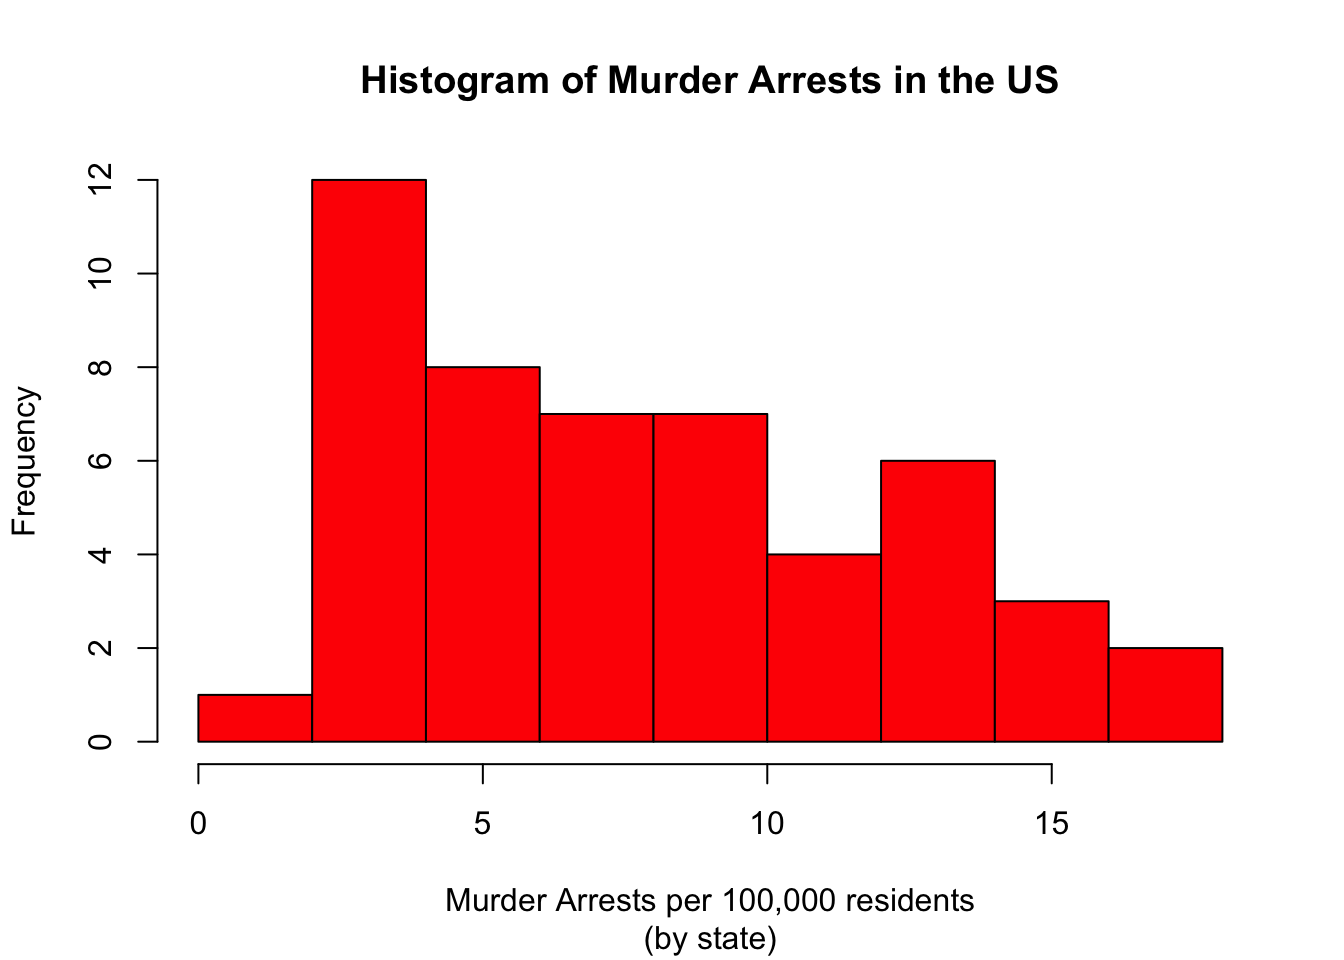
\includegraphics{Assignments_files/figure-latex/unnamed-chunk-6-1.pdf}

\hypertarget{problem-6}{%
\subsubsection{Problem 6}\label{problem-6}}

\emph{Please summarize \texttt{Murder} quantitatively. What are its mean
and median? What is the difference between mean and median? What is a
quartile, and why do you think R gives you the 1st Qu. and 3rd Qu.?}

\begin{Shaded}
\begin{Highlighting}[]
\FunctionTok{summary}\NormalTok{(dat}\SpecialCharTok{$}\NormalTok{Murder)}
\end{Highlighting}
\end{Shaded}

\begin{verbatim}
##    Min. 1st Qu.  Median    Mean 3rd Qu.    Max. 
##   0.800   4.075   7.250   7.788  11.250  17.400
\end{verbatim}

\textbf{Answer}: The mean of the Murder variable is 7.788 (murder
arrests per 100,000 residents of a state). The median is 7.250 (murder
arrests per 100,000 residents of a state). The difference between these
two values quantitatively is 0.538. The difference qualitatively is that
the mean represents the average number of murder arrests per 100,000
residents of all US states while the median is the middle value of the
data set, showing the data has a slight right skew. A quartile isdivides
the dataset into four parts, with Q1 being the median of the lower half
of the dataset and Q3 being the median of the upper half of the data
set. R gives you this information because quartiles can be helpful in
determining where a specific data point falls in the set; for example,
if a value for ``Murders'' is greater than Q3, 11.250, we can more
reasonably assume that this state has an exceptionally high murder rate
in comparison to other states in the US. If a state has a value for
``Murders'' that is less than 4.075, we can more reasonably assume that
this state is relatively safer than other US states!

\hypertarget{problem-7}{%
\subsubsection{Problem 7}\label{problem-7}}

\emph{Repeat the same steps you followed for \texttt{Murder}, for the
variables \texttt{Assault} and \texttt{Rape}. Now plot all three
histograms together. You can do this by using the command
\texttt{par(mfrow=c(3,1))} and then plotting each of the three. }

\begin{Shaded}
\begin{Highlighting}[]
\FunctionTok{hist}\NormalTok{(dat}\SpecialCharTok{$}\NormalTok{Assault, }\AttributeTok{col =} \StringTok{\textquotesingle{}red\textquotesingle{}}\NormalTok{, }\AttributeTok{ylab =} \StringTok{\textquotesingle{}Frequency\textquotesingle{}}\NormalTok{, }\AttributeTok{xlab =} \StringTok{\textquotesingle{}Assault Arrests per 100,000 residents\textquotesingle{}}\NormalTok{, }\AttributeTok{main =} \StringTok{\textquotesingle{}Histogram of Assault Arrests in the US\textquotesingle{}}\NormalTok{, }\AttributeTok{sub =} \StringTok{\textquotesingle{}(by state)\textquotesingle{}}\NormalTok{)}
\end{Highlighting}
\end{Shaded}

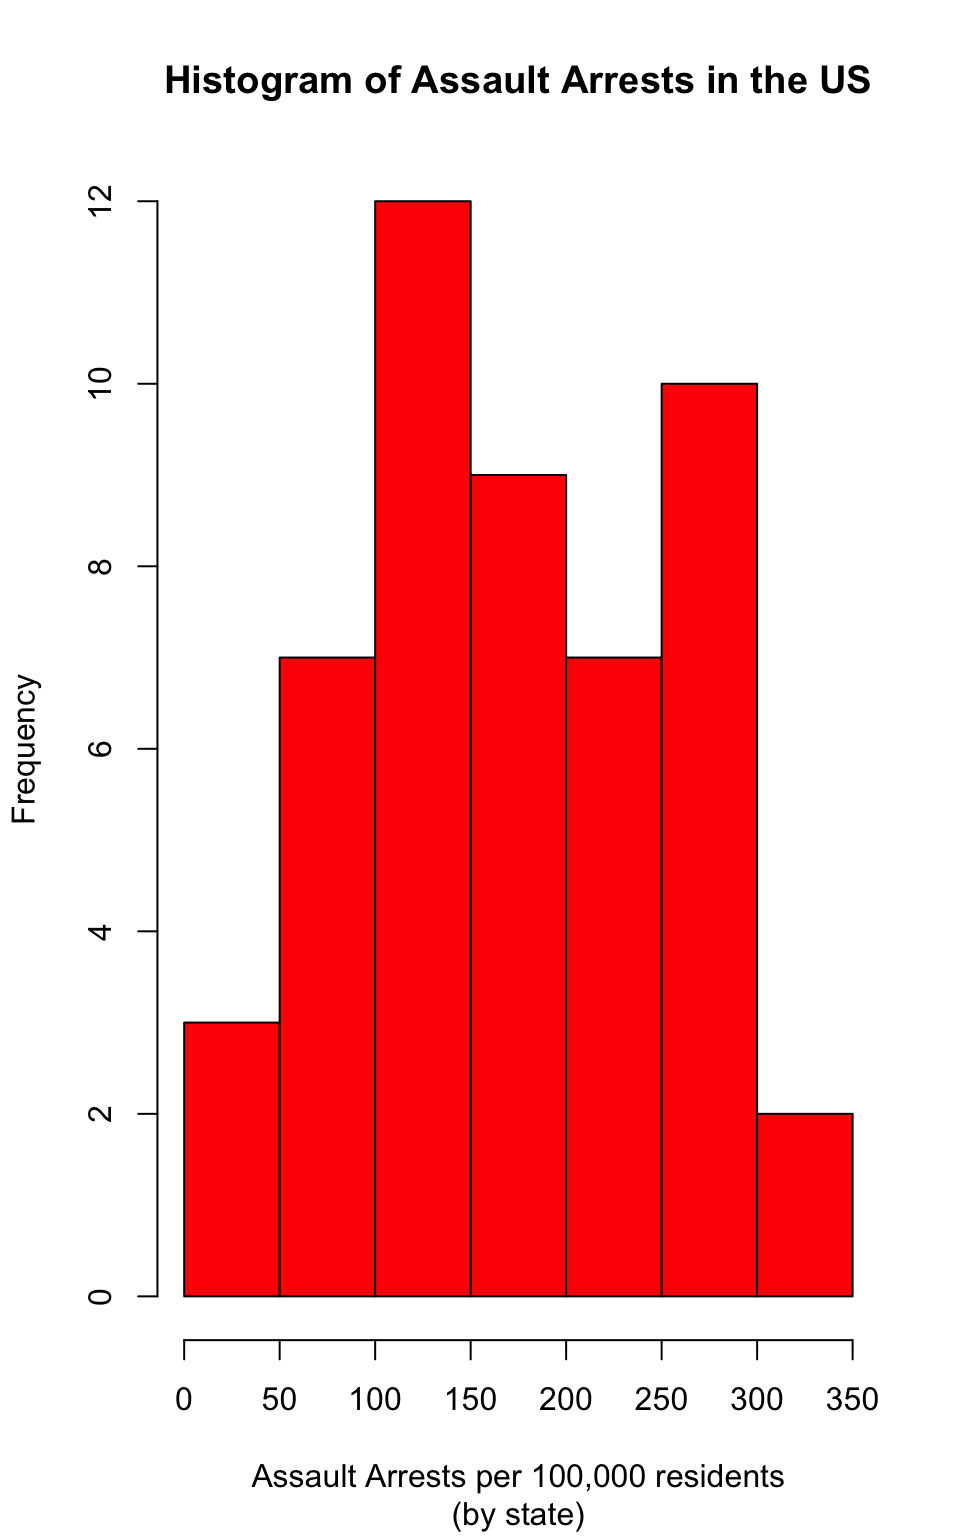
\includegraphics{Assignments_files/figure-latex/unnamed-chunk-8-1.pdf}

\begin{Shaded}
\begin{Highlighting}[]
\FunctionTok{summary}\NormalTok{(dat}\SpecialCharTok{$}\NormalTok{Assault)}
\end{Highlighting}
\end{Shaded}

\begin{verbatim}
##    Min. 1st Qu.  Median    Mean 3rd Qu.    Max. 
##    45.0   109.0   159.0   170.8   249.0   337.0
\end{verbatim}

\begin{Shaded}
\begin{Highlighting}[]
\FunctionTok{hist}\NormalTok{(dat}\SpecialCharTok{$}\NormalTok{Rape, }\AttributeTok{col =} \StringTok{\textquotesingle{}red\textquotesingle{}}\NormalTok{, }\AttributeTok{ylab =} \StringTok{\textquotesingle{}Frequency\textquotesingle{}}\NormalTok{, }\AttributeTok{xlab =} \StringTok{\textquotesingle{}Rape Arrests per 100,000 residents\textquotesingle{}}\NormalTok{, }\AttributeTok{main =} \StringTok{\textquotesingle{}Histogram of Rape Arrests in the US\textquotesingle{}}\NormalTok{, }\AttributeTok{sub =} \StringTok{\textquotesingle{}(by state)\textquotesingle{}}\NormalTok{)}
\end{Highlighting}
\end{Shaded}

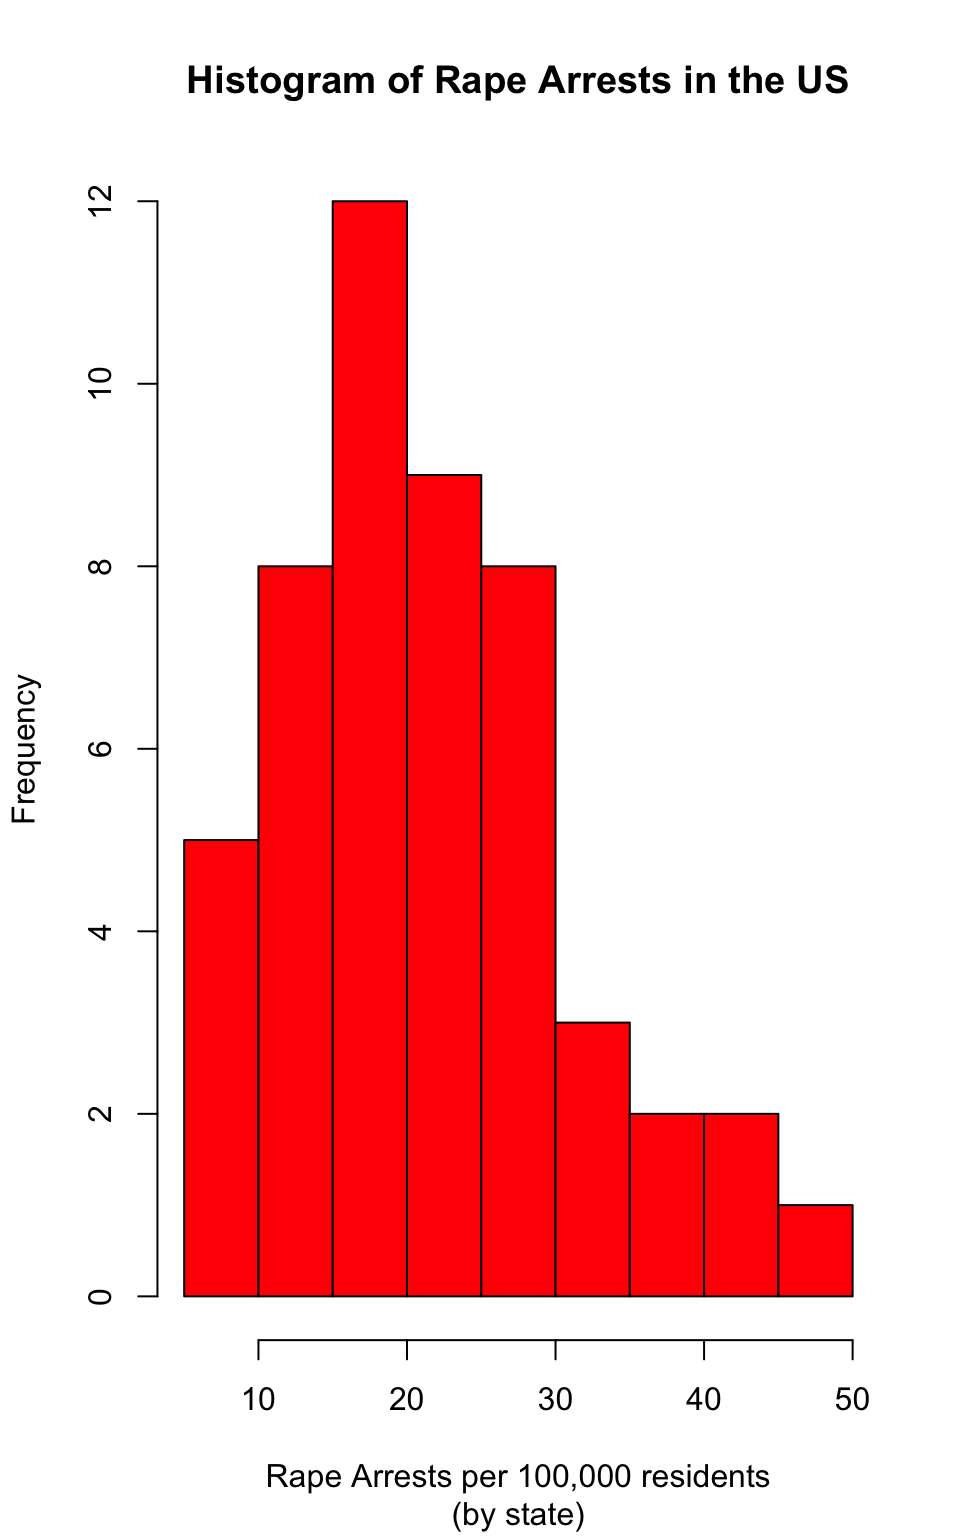
\includegraphics{Assignments_files/figure-latex/unnamed-chunk-8-2.pdf}

\begin{Shaded}
\begin{Highlighting}[]
\FunctionTok{summary}\NormalTok{(dat}\SpecialCharTok{$}\NormalTok{Rape)}
\end{Highlighting}
\end{Shaded}

\begin{verbatim}
##    Min. 1st Qu.  Median    Mean 3rd Qu.    Max. 
##    7.30   15.07   20.10   21.23   26.18   46.00
\end{verbatim}

\begin{Shaded}
\begin{Highlighting}[]
\FunctionTok{par}\NormalTok{(}\AttributeTok{mfrow=}\FunctionTok{c}\NormalTok{(}\DecValTok{3}\NormalTok{,}\DecValTok{1}\NormalTok{))}
\FunctionTok{hist}\NormalTok{(dat}\SpecialCharTok{$}\NormalTok{Murder, }\AttributeTok{col =} \StringTok{\textquotesingle{}red\textquotesingle{}}\NormalTok{, }\AttributeTok{ylab =} \StringTok{\textquotesingle{}Frequency\textquotesingle{}}\NormalTok{, }\AttributeTok{xlab =} \StringTok{\textquotesingle{}Murder Arrests per 100,000 residents\textquotesingle{}}\NormalTok{, }\AttributeTok{main =} \StringTok{\textquotesingle{}Histogram of Murder Arrests in the US\textquotesingle{}}\NormalTok{, }\AttributeTok{sub =} \StringTok{\textquotesingle{}(by state)\textquotesingle{}}\NormalTok{)}
\FunctionTok{hist}\NormalTok{(dat}\SpecialCharTok{$}\NormalTok{Assault, }\AttributeTok{col =} \StringTok{\textquotesingle{}red\textquotesingle{}}\NormalTok{, }\AttributeTok{ylab =} \StringTok{\textquotesingle{}Frequency\textquotesingle{}}\NormalTok{, }\AttributeTok{xlab =} \StringTok{\textquotesingle{}Assault Arrests per 100,000 residents\textquotesingle{}}\NormalTok{, }\AttributeTok{main =} \StringTok{\textquotesingle{}Histogram of Assault Arrests in the US\textquotesingle{}}\NormalTok{, }\AttributeTok{sub =} \StringTok{\textquotesingle{}(by state)\textquotesingle{}}\NormalTok{)}
\FunctionTok{summary}\NormalTok{(dat}\SpecialCharTok{$}\NormalTok{Assault)}
\end{Highlighting}
\end{Shaded}

\begin{verbatim}
##    Min. 1st Qu.  Median    Mean 3rd Qu.    Max. 
##    45.0   109.0   159.0   170.8   249.0   337.0
\end{verbatim}

\begin{Shaded}
\begin{Highlighting}[]
\FunctionTok{hist}\NormalTok{(dat}\SpecialCharTok{$}\NormalTok{Rape, }\AttributeTok{col =} \StringTok{\textquotesingle{}red\textquotesingle{}}\NormalTok{, }\AttributeTok{ylab =} \StringTok{\textquotesingle{}Frequency\textquotesingle{}}\NormalTok{, }\AttributeTok{xlab =} \StringTok{\textquotesingle{}Rape Arrests per 100,000 residents\textquotesingle{}}\NormalTok{, }\AttributeTok{main =} \StringTok{\textquotesingle{}Histogram of Rape Arrests in the US\textquotesingle{}}\NormalTok{, }\AttributeTok{sub =} \StringTok{\textquotesingle{}(by state)\textquotesingle{}}\NormalTok{)}
\end{Highlighting}
\end{Shaded}

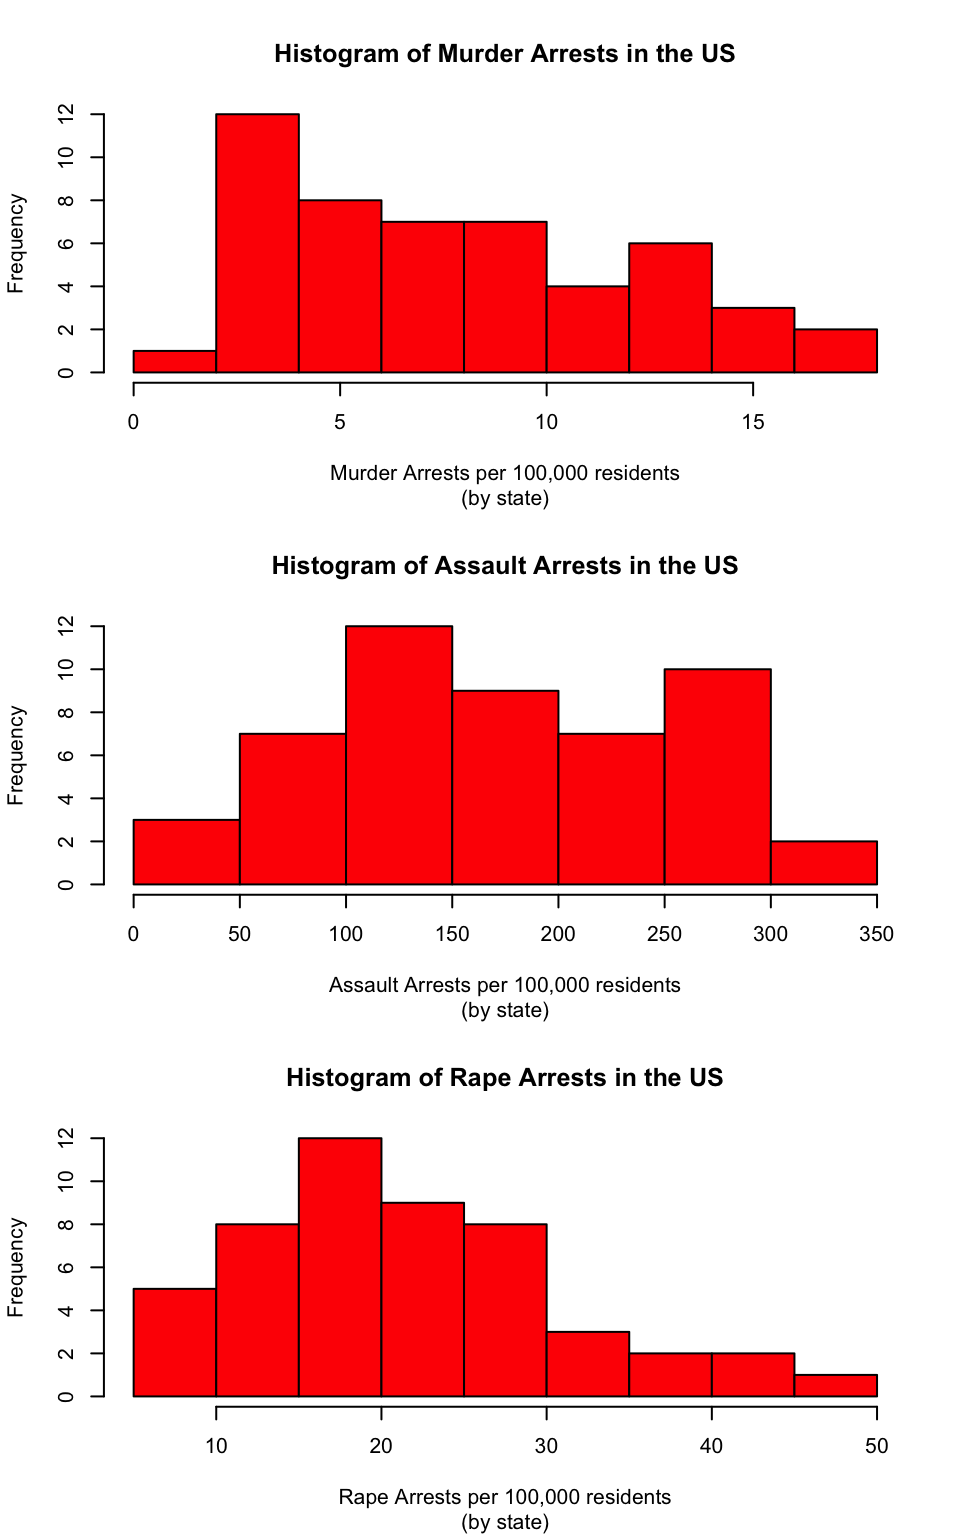
\includegraphics{Assignments_files/figure-latex/unnamed-chunk-8-3.pdf}

\emph{What does the command par do, in your own words (you can look this
up by asking R \texttt{?par})?}

\textbf{Answer}: The par function allows an R user to look at the
graphical parameters that control how graphs are displayed. In the case
of the par(mfrow=c(3,1)) function, we are able to not only look at the
graphical parameters, but control them so that we can decide how many
subplots we want displayed.

\emph{What can you learn from plotting the histograms together?}

\textbf{Answer}: From plotting the histograms together, we can view a
comparison of the distributions in relation to each other, examining
skew and quartile arrangement to see how distributions vary by crime
type. On a more general note, plotting the histograms together allows us
to see generally how frequency and distribution relationships among
multiple variables interact, allowing a viewer a more clear image of the
relationship between variables while still being able to view a more
individualistic look at each histogram.

\hypertarget{problem-8}{%
\subsubsection{Problem 8}\label{problem-8}}

\emph{In the console below (not in text), type
\texttt{install.packages("maps")} and press Enter, and then type
\texttt{install.packages("ggplot2")} and press Enter. This will install
the packages so you can load the libraries.}

\emph{Run this code:}

\begin{Shaded}
\begin{Highlighting}[]
\FunctionTok{library}\NormalTok{(maps) }
\FunctionTok{library}\NormalTok{(ggplot2) }

\FunctionTok{ggplot}\NormalTok{(dat, }\FunctionTok{aes}\NormalTok{(}\AttributeTok{map\_id=}\NormalTok{state, }\AttributeTok{fill=}\NormalTok{Murder)) }\SpecialCharTok{+} 
  \FunctionTok{geom\_map}\NormalTok{(}\AttributeTok{map=}\FunctionTok{map\_data}\NormalTok{(}\StringTok{"state"}\NormalTok{)) }\SpecialCharTok{+} 
  \FunctionTok{expand\_limits}\NormalTok{(}\AttributeTok{x=}\FunctionTok{map\_data}\NormalTok{(}\StringTok{"state"}\NormalTok{)}\SpecialCharTok{$}\NormalTok{long, }\AttributeTok{y=}\FunctionTok{map\_data}\NormalTok{(}\StringTok{"state"}\NormalTok{)}\SpecialCharTok{$}\NormalTok{lat)}
\end{Highlighting}
\end{Shaded}

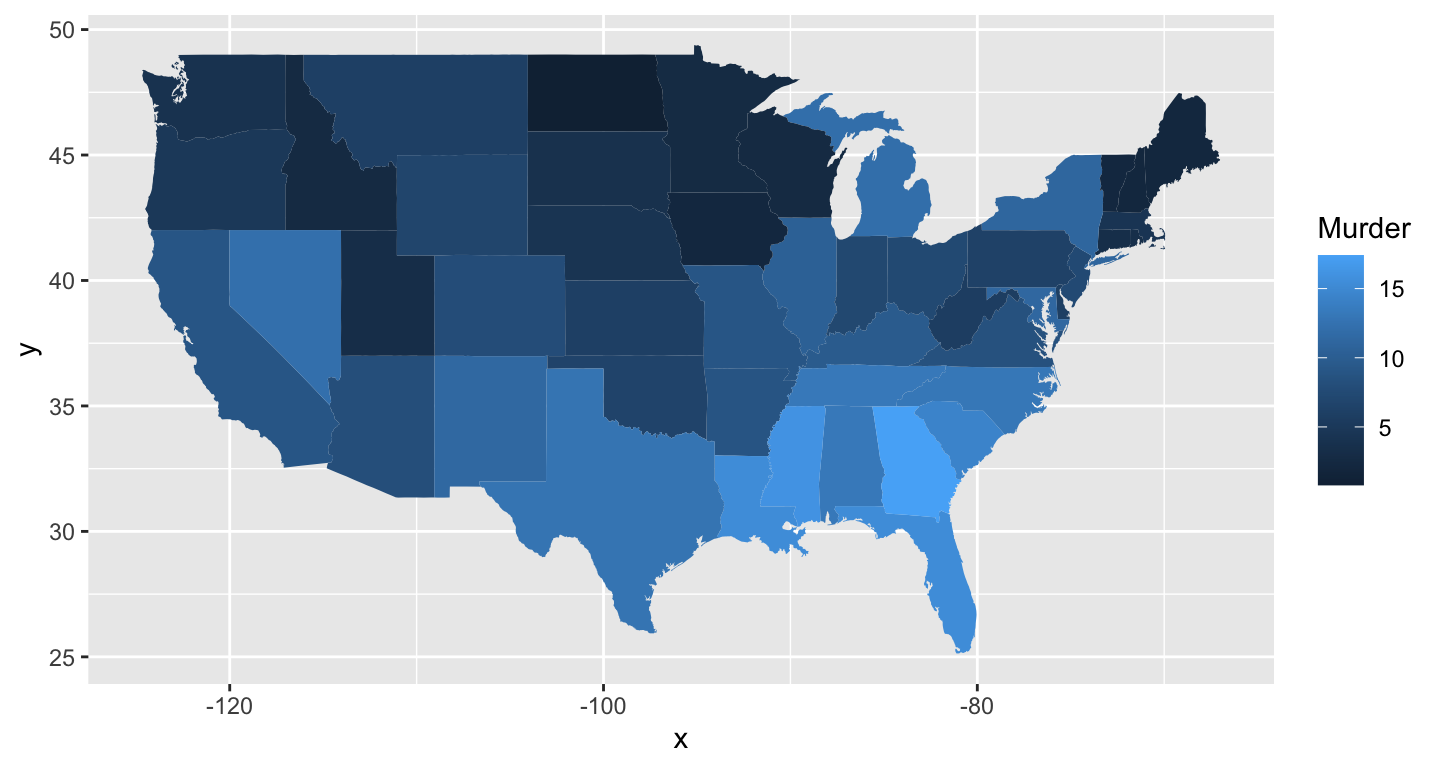
\includegraphics{Assignments_files/figure-latex/unnamed-chunk-9-1.pdf}

\emph{What does this code do? Explain what each line is doing.}

\textbf{Answer}: ggplot is the most basic implementation of any data
visualization in R. In this instance, the first line of code is filling
out the basic information of the data visual by specifying the variables
which are involved in the plot. The second line of code employs the maps
package and ggplot2 package to choose specifically to create a mapping
of the selected variables, using states as the selected implementation
of the map. The third line employs the expand\_limit function in order
to ensure that the limits of the visualization include a single value
for all aspects of the plot, implying what should be included in the
scale.

\[\\[2in]\]

\hypertarget{assignment-2}{%
\section{Assignment 2}\label{assignment-2}}

Instructions: Copy your code, paste it into a Word document, and turn it
into Canvas. You can turn in a .docx or .pdf file. Show any EDA
(graphical or non-graphical) you have used to come to this conclusion.

\hypertarget{problem-1-load-data}{%
\subsection{Problem 1: Load data}\label{problem-1-load-data}}

Set your working directory to the folder where you downloaded the data.

\begin{Shaded}
\begin{Highlighting}[]
\FunctionTok{setwd}\NormalTok{(}\StringTok{"\textasciitilde{}/Documents/GitHub/SophieCRIM250"}\NormalTok{)}
\end{Highlighting}
\end{Shaded}

Read the data

\begin{Shaded}
\begin{Highlighting}[]
\NormalTok{dat }\OtherTok{\textless{}{-}} \FunctionTok{read.csv}\NormalTok{(}\AttributeTok{file =} \StringTok{\textquotesingle{}dat.nsduh.small.1.csv\textquotesingle{}}\NormalTok{)}
\end{Highlighting}
\end{Shaded}

What are the dimensions of the dataset?

\begin{Shaded}
\begin{Highlighting}[]
\FunctionTok{names}\NormalTok{(dat)}
\end{Highlighting}
\end{Shaded}

\begin{verbatim}
## [1] "mjage"     "cigage"    "iralcage"  "age2"      "sexatract" "speakengl"
## [7] "irsex"
\end{verbatim}

\begin{Shaded}
\begin{Highlighting}[]
\FunctionTok{dim}\NormalTok{(dat)}
\end{Highlighting}
\end{Shaded}

\begin{verbatim}
## [1] 171   7
\end{verbatim}

\begin{itemize}
\tightlist
\item
  The dimensions are 171 x 7
\end{itemize}

\hypertarget{problem-2-variables}{%
\subsection{Problem 2: Variables}\label{problem-2-variables}}

Describe the variables in the dataset. - mjage is a variable that
denotes how old someone was the first time they used marijuana or
hashish - cigage is a variable that denotes how old someone was when
they first started smoking cigarettes every day - iralcage is a variable
that denotes how old someone was when they first tried alcohol, numbers
greater than 900 implying never used or lack of answer - age2 is a
variable that splits people up into groups based on respondent age -
sexatract is a variable that splits people into groups based on sexual
attraction, each number denoting a different sexual preference -
speakengl is a variable that splits people into groups based off of
their english literacy - irsex is a variable that splits people into two
different groups based on a binary gender system, 1 being male and 2
being female

What is this dataset about? Who collected the data, what kind of sample
is it, and what was the purpose of generating the data? - This dataset
is about the health and drug use statistics of the United States. - This
data is from the National Survey on Drug Use and Health, conducted by
The Substance Abuse and Mental Health Services Administration in the US
Department of Health and Human Services. - This is a random sample. -
The data was generated for the sake of government agencies, private
organizations, individual researchers, and the public at large for a
number of different purposes. - This data is used mainly to provide more
information on substance use and demographic statistics in the United
States.

\hypertarget{problem-3-age-and-gender}{%
\subsection{Problem 3: Age and gender}\label{problem-3-age-and-gender}}

What is the age distribution of the sample like? Make sure you read the
codebook to know what the variable values mean.

\begin{Shaded}
\begin{Highlighting}[]
\FunctionTok{hist}\NormalTok{(dat}\SpecialCharTok{$}\NormalTok{age2)}
\end{Highlighting}
\end{Shaded}

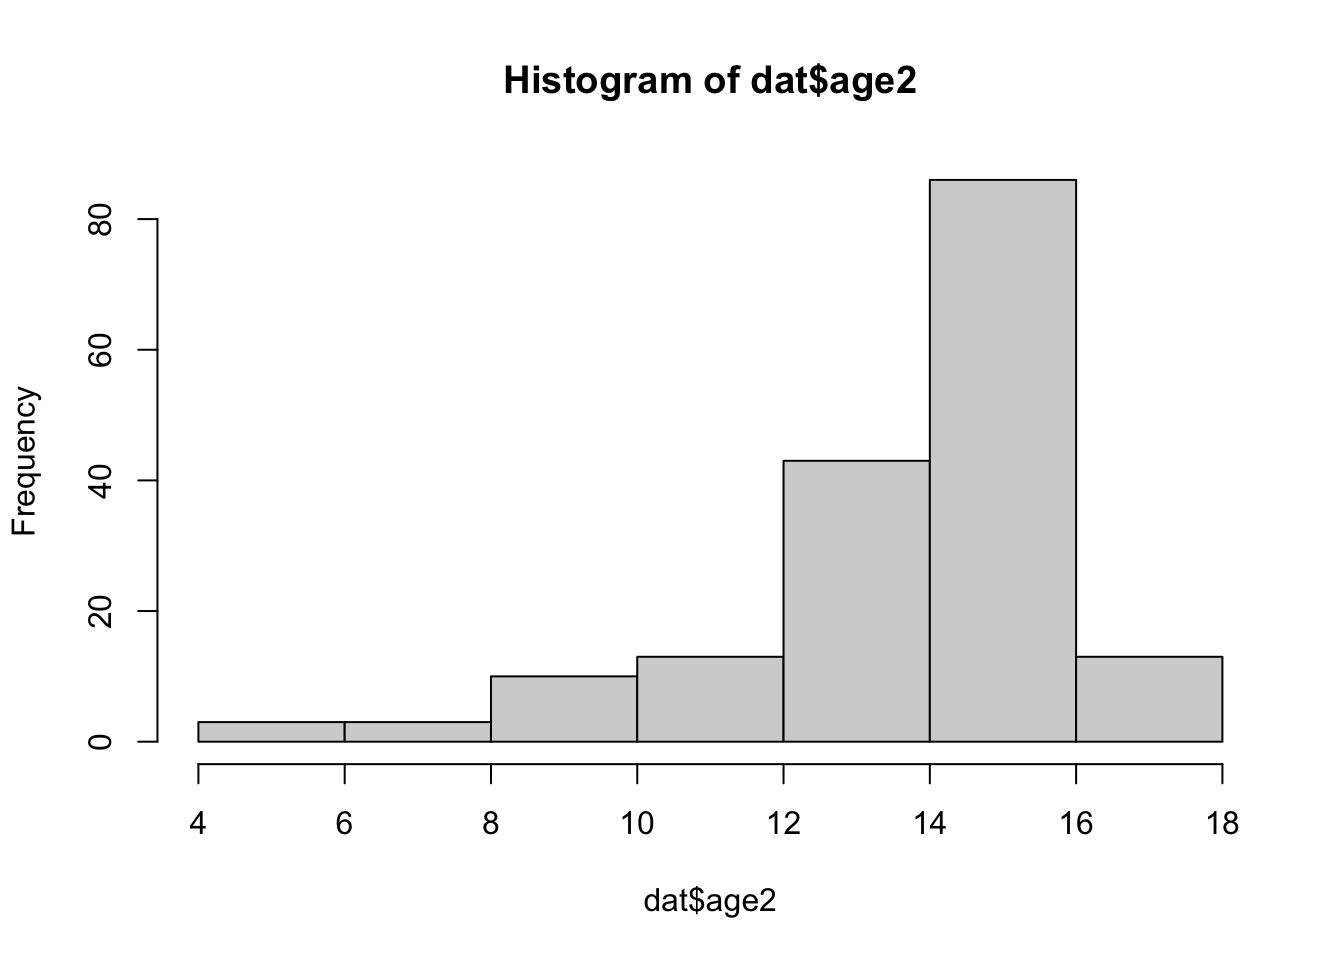
\includegraphics{Assignments_files/figure-latex/unnamed-chunk-13-1.pdf}

\begin{Shaded}
\begin{Highlighting}[]
\FunctionTok{summary}\NormalTok{(dat}\SpecialCharTok{$}\NormalTok{age2)}
\end{Highlighting}
\end{Shaded}

\begin{verbatim}
##    Min. 1st Qu.  Median    Mean 3rd Qu.    Max. 
##    4.00   13.00   15.00   13.98   15.00   17.00
\end{verbatim}

\begin{itemize}
\tightlist
\item
  The age distribution is left skewed, with a mean of 13.98
  (representing ages 26-29) and median of 15 (representing ages 35-49).
  \# Do you think this age distribution representative of the US
  population? Why or why not?
\item
  I do feel like this sample is representative. The distribution of ages
  in the age set are misleading; the ages of 18-49 (as represented by
  groups 7-15) are the majority of the sample, which is consistent with
  the most recent US Census. \# Is the sample balanced in terms of
  gender? If not, are there more females or males?
\end{itemize}

\begin{Shaded}
\begin{Highlighting}[]
\FunctionTok{summary}\NormalTok{(dat}\SpecialCharTok{$}\NormalTok{irsex)}
\end{Highlighting}
\end{Shaded}

\begin{verbatim}
##    Min. 1st Qu.  Median    Mean 3rd Qu.    Max. 
##   1.000   1.000   1.000   1.468   2.000   2.000
\end{verbatim}

\begin{itemize}
\tightlist
\item
  This sample is fairly balanced in terms of gender. The mean for the
  irsex variable is 1.468, meaning the sample is fairly balanced in
  terms of sex. \# Use this code to draw a stacked bar plot to view the
  relationship between sex and age. What can you conclude from this
  plot?
\end{itemize}

\begin{Shaded}
\begin{Highlighting}[]
\NormalTok{tab.agesex }\OtherTok{\textless{}{-}} \FunctionTok{table}\NormalTok{(dat}\SpecialCharTok{$}\NormalTok{irsex, dat}\SpecialCharTok{$}\NormalTok{age2)}
\FunctionTok{barplot}\NormalTok{(tab.agesex,}
        \AttributeTok{main =} \StringTok{"Stacked barchart"}\NormalTok{,}
        \AttributeTok{xlab =} \StringTok{"Age category"}\NormalTok{, }\AttributeTok{ylab =} \StringTok{"Frequency"}\NormalTok{,}
        \AttributeTok{legend.text =} \FunctionTok{rownames}\NormalTok{(tab.agesex),}
        \AttributeTok{beside =} \ConstantTok{FALSE}\NormalTok{) }\CommentTok{\# Stacked bars (default)}
\end{Highlighting}
\end{Shaded}

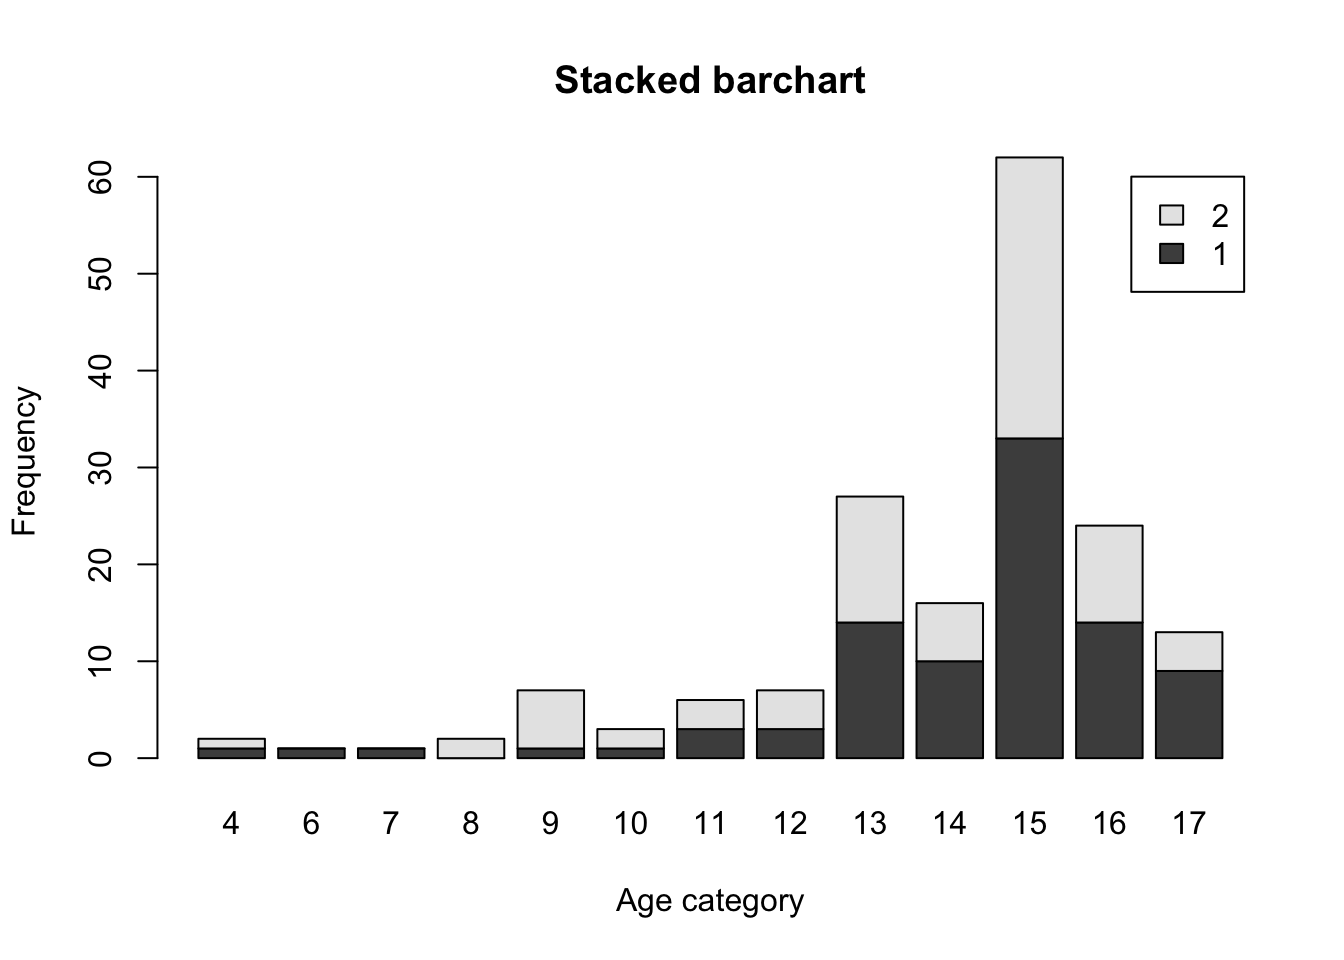
\includegraphics{Assignments_files/figure-latex/unnamed-chunk-15-1.pdf}
- This plot demonstrates that the distribution is fairly balanced in
age, with the majority of participants on either tail of the data being
mainly males.

\hypertarget{problem-4-substance-use}{%
\subsection{Problem 4: Substance use}\label{problem-4-substance-use}}

For which of the three substances included in the dataset (marijuana,
alcohol, and cigarettes) do individuals tend to use the substance
earlier?

\begin{Shaded}
\begin{Highlighting}[]
\FunctionTok{par}\NormalTok{(}\AttributeTok{mfrow=}\FunctionTok{c}\NormalTok{(}\DecValTok{3}\NormalTok{,}\DecValTok{1}\NormalTok{))}
\FunctionTok{hist}\NormalTok{(dat}\SpecialCharTok{$}\NormalTok{mjage, }\AttributeTok{col =} \StringTok{\textquotesingle{}red\textquotesingle{}}\NormalTok{, }\AttributeTok{ylab =} \StringTok{\textquotesingle{}Frequency\textquotesingle{}}\NormalTok{, }\AttributeTok{xlab =} \StringTok{\textquotesingle{}Age category\textquotesingle{}}\NormalTok{, }\AttributeTok{main =} \StringTok{\textquotesingle{}Histogram of Marijuana Usage\textquotesingle{}}\NormalTok{)}
\FunctionTok{hist}\NormalTok{(dat}\SpecialCharTok{$}\NormalTok{cigage , }\AttributeTok{col =} \StringTok{\textquotesingle{}red\textquotesingle{}}\NormalTok{, }\AttributeTok{ylab =} \StringTok{\textquotesingle{}Frequency\textquotesingle{}}\NormalTok{, }\AttributeTok{xlab =} \StringTok{\textquotesingle{}Age category\textquotesingle{}}\NormalTok{, }\AttributeTok{main =} \StringTok{\textquotesingle{}Histogram of Cigarette Usage\textquotesingle{}}\NormalTok{)}
\FunctionTok{hist}\NormalTok{(dat}\SpecialCharTok{$}\NormalTok{iralcage, }\AttributeTok{col =} \StringTok{\textquotesingle{}red\textquotesingle{}}\NormalTok{, }\AttributeTok{ylab =} \StringTok{\textquotesingle{}Frequency\textquotesingle{}}\NormalTok{, }\AttributeTok{xlab =} \StringTok{\textquotesingle{}Age category\textquotesingle{}}\NormalTok{, }\AttributeTok{main =} \StringTok{\textquotesingle{}Histogram of Alcohol Consumption\textquotesingle{}}\NormalTok{)}
\end{Highlighting}
\end{Shaded}

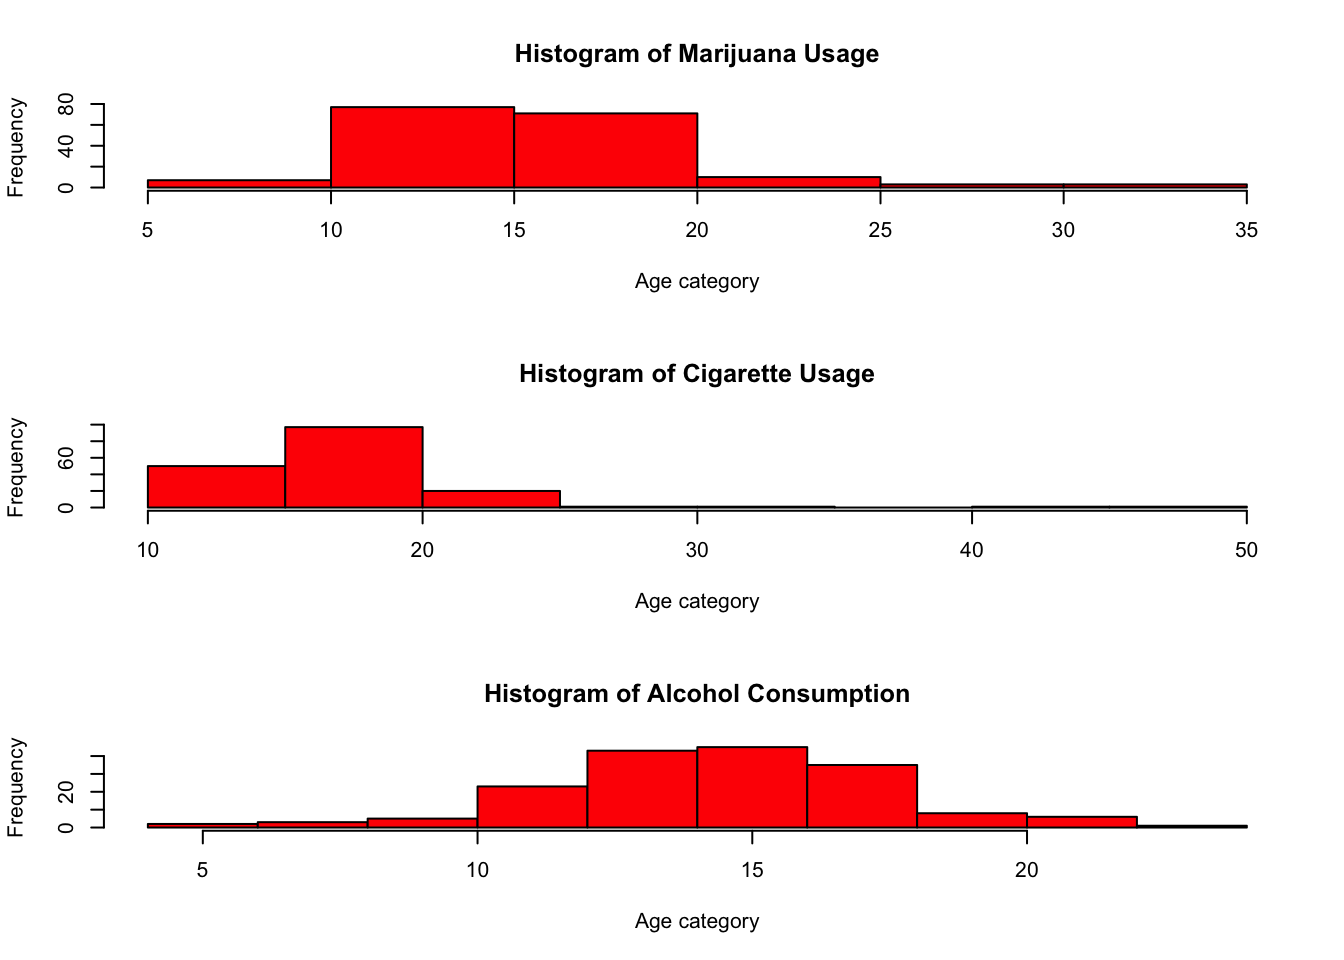
\includegraphics{Assignments_files/figure-latex/unnamed-chunk-16-1.pdf}
- Individuals tend to use marijuana at the youngest age out of the three
substances.

\hypertarget{problem-5-sexual-attraction}{%
\subsection{Problem 5: Sexual
attraction}\label{problem-5-sexual-attraction}}

\begin{Shaded}
\begin{Highlighting}[]
\FunctionTok{library}\NormalTok{(ggplot2)}
\end{Highlighting}
\end{Shaded}

\hypertarget{what-does-the-distribution-of-sexual-attraction-look-like-is-this-what-you-expected}{%
\subsection{What does the distribution of sexual attraction look like?
Is this what you
expected?}\label{what-does-the-distribution-of-sexual-attraction-look-like-is-this-what-you-expected}}

\begin{Shaded}
\begin{Highlighting}[]
\FunctionTok{hist}\NormalTok{(dat}\SpecialCharTok{$}\NormalTok{sexatract)}
\end{Highlighting}
\end{Shaded}

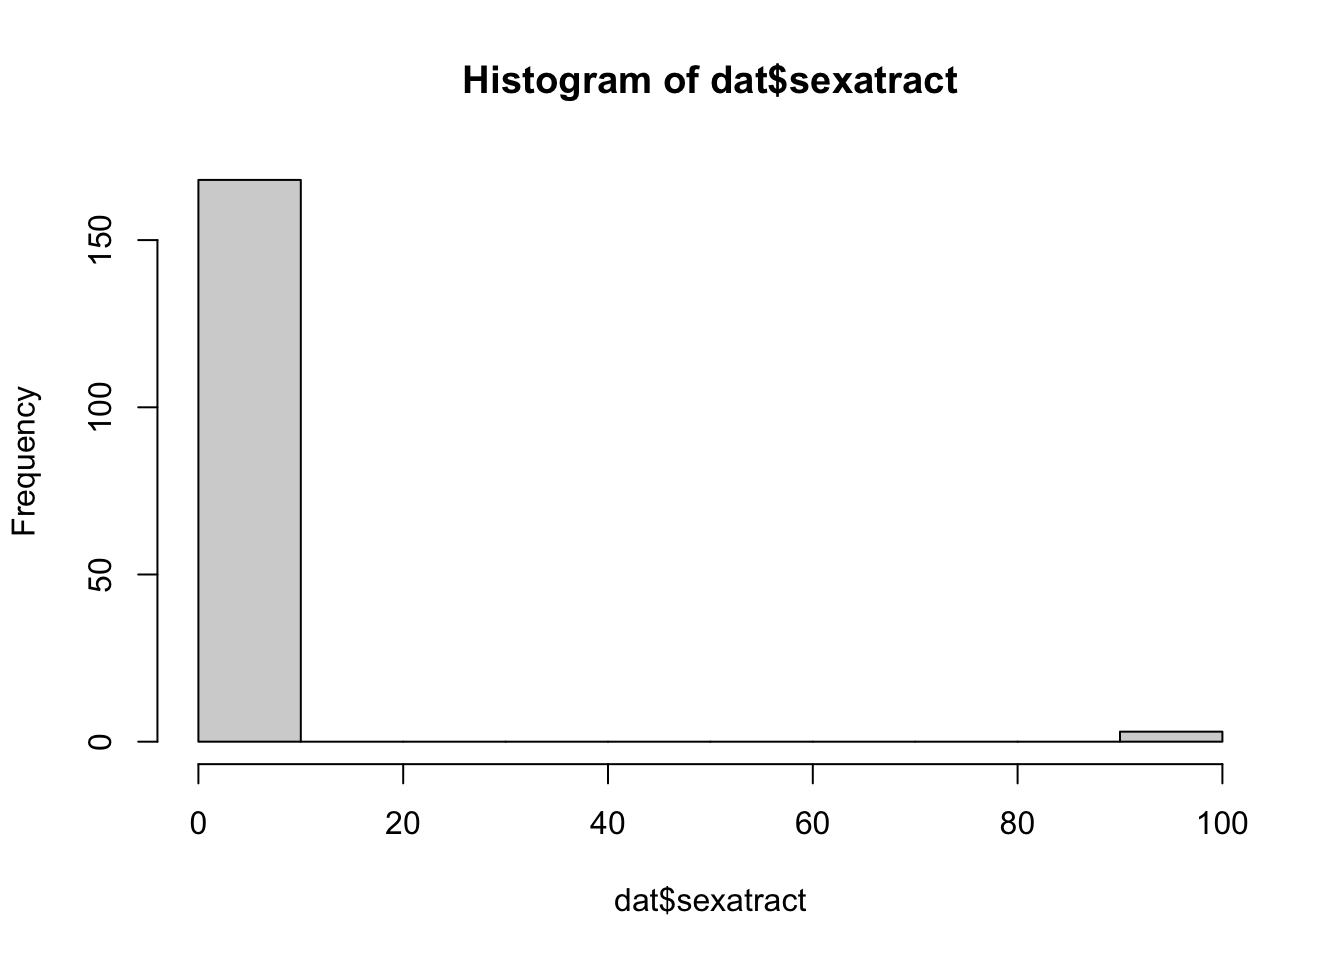
\includegraphics{Assignments_files/figure-latex/unnamed-chunk-18-1.pdf}

\begin{Shaded}
\begin{Highlighting}[]
\FunctionTok{summary}\NormalTok{(dat}\SpecialCharTok{$}\NormalTok{sexatract)}
\end{Highlighting}
\end{Shaded}

\begin{verbatim}
##    Min. 1st Qu.  Median    Mean 3rd Qu.    Max. 
##    1.00    1.00    1.00    3.07    1.00   99.00
\end{verbatim}

\begin{Shaded}
\begin{Highlighting}[]
\FunctionTok{table}\NormalTok{(dat}\SpecialCharTok{$}\NormalTok{sexatract)}
\end{Highlighting}
\end{Shaded}

\begin{verbatim}
## 
##   1   2   3   4   5   6  99 
## 136  16   9   3   3   1   3
\end{verbatim}

\begin{itemize}
\tightlist
\item
  According to the numeric system for sexual attraction, this gives the
  distribution a strong right skew.
\item
  This is not a necessarily surprising result, considering there is
  generally a strong heterosexual representation in the United States,
  especially on representative surveys.
\item
  While I do not feel this is truly representative of the United States,
  there are many people who may feel uncomfortable correctly identifying
  sexual preference on a survey used by government organizations and
  regarding personal information (even if it is later encoded).
\end{itemize}

\hypertarget{what-is-the-distribution-of-sexual-attraction-by-gender}{%
\subsection{What is the distribution of sexual attraction by
gender?}\label{what-is-the-distribution-of-sexual-attraction-by-gender}}

\begin{Shaded}
\begin{Highlighting}[]
\NormalTok{genatt }\OtherTok{\textless{}{-}} \FunctionTok{table}\NormalTok{(dat}\SpecialCharTok{$}\NormalTok{irsex, dat}\SpecialCharTok{$}\NormalTok{sexatract)}
\FunctionTok{barplot}\NormalTok{(genatt,}
        \AttributeTok{main =} \StringTok{"Stacked barchart"}\NormalTok{,}
        \AttributeTok{xlab =} \StringTok{"Gender"}\NormalTok{, }\AttributeTok{ylab =} \StringTok{"Frequency"}\NormalTok{,}
        \AttributeTok{legend.text =} \FunctionTok{rownames}\NormalTok{(genatt),}
        \AttributeTok{beside =} \ConstantTok{FALSE}\NormalTok{) }\CommentTok{\# Stacked bars (default)}
\end{Highlighting}
\end{Shaded}

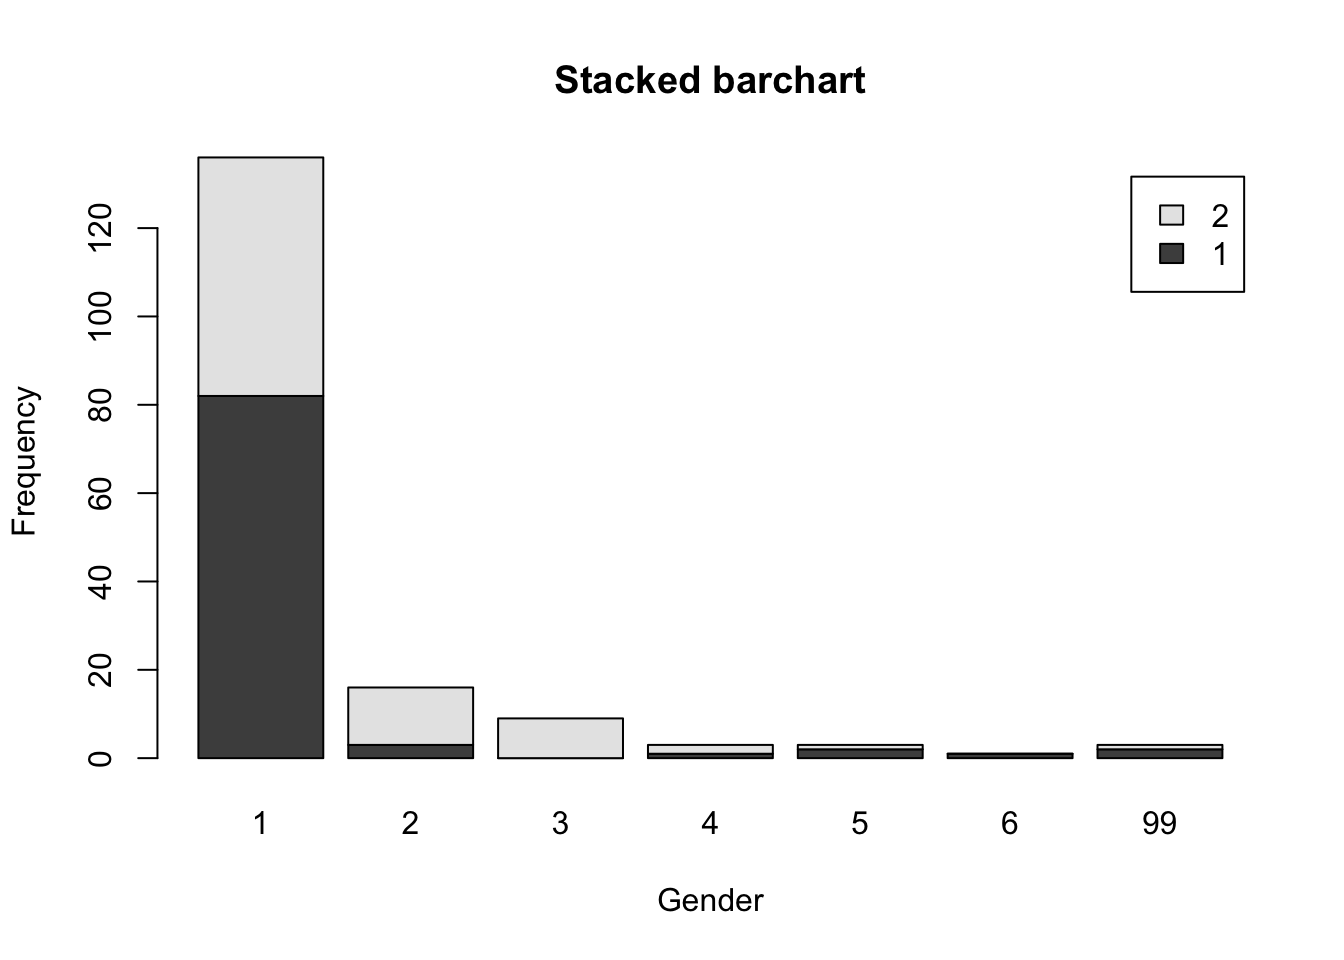
\includegraphics{Assignments_files/figure-latex/unnamed-chunk-19-1.pdf}

\begin{Shaded}
\begin{Highlighting}[]
\FunctionTok{sum}\NormalTok{(dat}\SpecialCharTok{$}\NormalTok{sexatract }\SpecialCharTok{==} \DecValTok{1} \SpecialCharTok{\&}\NormalTok{ dat}\SpecialCharTok{$}\NormalTok{irsex }\SpecialCharTok{==} \DecValTok{1}\NormalTok{)}
\end{Highlighting}
\end{Shaded}

\begin{verbatim}
## [1] 82
\end{verbatim}

\begin{Shaded}
\begin{Highlighting}[]
\SpecialCharTok{{-}} \DecValTok{82}
\end{Highlighting}
\end{Shaded}

\begin{verbatim}
## [1] -82
\end{verbatim}

\begin{Shaded}
\begin{Highlighting}[]
\FunctionTok{sum}\NormalTok{(dat}\SpecialCharTok{$}\NormalTok{sexatract }\SpecialCharTok{==} \DecValTok{1} \SpecialCharTok{\&}\NormalTok{ dat}\SpecialCharTok{$}\NormalTok{irsex }\SpecialCharTok{==} \DecValTok{2}\NormalTok{)}
\end{Highlighting}
\end{Shaded}

\begin{verbatim}
## [1] 54
\end{verbatim}

\begin{Shaded}
\begin{Highlighting}[]
\SpecialCharTok{{-}} \DecValTok{54}
\end{Highlighting}
\end{Shaded}

\begin{verbatim}
## [1] -54
\end{verbatim}

\begin{itemize}
\tightlist
\item
  The distribution of sexual attraction is highly populated by those who
  identified (via the codebook) as only being attracted to the opposite
  gender.
\item
  A smaller number of women identify as being heterosexual than men,
  thought this could be slightly biased due to a smaller sample size of
  women. \#\# Problem 6: English speaking
\end{itemize}

What does the distribution of English speaking look like in the sample?
Is this what you might expect for a random sample of the US population?
summary(dat\(speakengl) table(dat\)speakengl) - Majority of the sample
are English speakers, with 169 of the 171 respondents self-identifying
as speaking English well or very well and only two respondents not
speaking English well. - This is not what I would expect from a random
sample of the US, but makes sense in the fact that this is a survey
administered in English, probably leading to some sampling bias in a
high yield of English speakers. Are there more English speaker females
or males?

\begin{Shaded}
\begin{Highlighting}[]
\FunctionTok{sum}\NormalTok{(dat}\SpecialCharTok{$}\NormalTok{speakengl }\SpecialCharTok{==} \DecValTok{1} \SpecialCharTok{\&}\NormalTok{ dat}\SpecialCharTok{$}\NormalTok{irsex }\SpecialCharTok{==} \DecValTok{1}\NormalTok{)}
\end{Highlighting}
\end{Shaded}

\begin{verbatim}
## [1] 84
\end{verbatim}

\begin{Shaded}
\begin{Highlighting}[]
\SpecialCharTok{{-}} \DecValTok{84}
\end{Highlighting}
\end{Shaded}

\begin{verbatim}
## [1] -84
\end{verbatim}

\begin{Shaded}
\begin{Highlighting}[]
\FunctionTok{sum}\NormalTok{(dat}\SpecialCharTok{$}\NormalTok{speakengl }\SpecialCharTok{==} \DecValTok{1} \SpecialCharTok{\&}\NormalTok{ dat}\SpecialCharTok{$}\NormalTok{irsex }\SpecialCharTok{==} \DecValTok{2}\NormalTok{)}
\end{Highlighting}
\end{Shaded}

\begin{verbatim}
## [1] 77
\end{verbatim}

\begin{Shaded}
\begin{Highlighting}[]
\SpecialCharTok{{-}} \DecValTok{77}
\end{Highlighting}
\end{Shaded}

\begin{verbatim}
## [1] -77
\end{verbatim}

\begin{Shaded}
\begin{Highlighting}[]
\FunctionTok{sum}\NormalTok{(dat}\SpecialCharTok{$}\NormalTok{speakengl }\SpecialCharTok{==} \DecValTok{2} \SpecialCharTok{\&}\NormalTok{ dat}\SpecialCharTok{$}\NormalTok{irsex }\SpecialCharTok{==} \DecValTok{1}\NormalTok{)}
\end{Highlighting}
\end{Shaded}

\begin{verbatim}
## [1] 7
\end{verbatim}

\begin{Shaded}
\begin{Highlighting}[]
\SpecialCharTok{{-}} \DecValTok{7}
\end{Highlighting}
\end{Shaded}

\begin{verbatim}
## [1] -7
\end{verbatim}

\begin{Shaded}
\begin{Highlighting}[]
\FunctionTok{sum}\NormalTok{(dat}\SpecialCharTok{$}\NormalTok{speakengl }\SpecialCharTok{==} \DecValTok{2} \SpecialCharTok{\&}\NormalTok{ dat}\SpecialCharTok{$}\NormalTok{irsex }\SpecialCharTok{==} \DecValTok{2}\NormalTok{)}
\end{Highlighting}
\end{Shaded}

\begin{verbatim}
## [1] 1
\end{verbatim}

\begin{Shaded}
\begin{Highlighting}[]
\SpecialCharTok{{-}} \DecValTok{1}
\end{Highlighting}
\end{Shaded}

\begin{verbatim}
## [1] -1
\end{verbatim}

\begin{Shaded}
\begin{Highlighting}[]
\FunctionTok{sum}\NormalTok{(dat}\SpecialCharTok{$}\NormalTok{speakengl }\SpecialCharTok{==} \DecValTok{3} \SpecialCharTok{\&}\NormalTok{ dat}\SpecialCharTok{$}\NormalTok{irsex }\SpecialCharTok{==} \DecValTok{1}\NormalTok{)}
\end{Highlighting}
\end{Shaded}

\begin{verbatim}
## [1] 0
\end{verbatim}

\begin{Shaded}
\begin{Highlighting}[]
\SpecialCharTok{{-}} \DecValTok{0}
\end{Highlighting}
\end{Shaded}

\begin{verbatim}
## [1] 0
\end{verbatim}

\begin{Shaded}
\begin{Highlighting}[]
\FunctionTok{sum}\NormalTok{(dat}\SpecialCharTok{$}\NormalTok{speakengl }\SpecialCharTok{==} \DecValTok{3} \SpecialCharTok{\&}\NormalTok{ dat}\SpecialCharTok{$}\NormalTok{irsex }\SpecialCharTok{==} \DecValTok{2}\NormalTok{)}
\end{Highlighting}
\end{Shaded}

\begin{verbatim}
## [1] 2
\end{verbatim}

\begin{Shaded}
\begin{Highlighting}[]
\SpecialCharTok{{-}} \DecValTok{2}
\end{Highlighting}
\end{Shaded}

\begin{verbatim}
## [1] -2
\end{verbatim}

\begin{itemize}
\tightlist
\item
  Assuming that we say that ``not an English speaker'' is characterized
  by someone self-assessing themselves as speaking English ``not well,''
  there is a higher number of female non-English speakers.
\item
  This means that, from this very limited data set, there is a higher
  number of male English speakers.
\end{itemize}

\hypertarget{exam-1}{%
\section{Exam 1}\label{exam-1}}

\hypertarget{instructions}{%
\subsection{Instructions}\label{instructions}}

\begin{enumerate}
\def\labelenumi{\alph{enumi}.}
\item
  Create a folder in your computer (a good place would be under Crim
  250, Exams).
\item
  Download the dataset from the Canvas website
  (fatal-police-shootings-data.csv) onto that folder, and save your Exam
  1.Rmd file in the same folder.
\item
  Download the README.md file. This is the codebook.
\item
  Load the data into an R data frame.
\end{enumerate}

\begin{Shaded}
\begin{Highlighting}[]
\NormalTok{dat }\OtherTok{\textless{}{-}} \FunctionTok{read.csv}\NormalTok{(}\StringTok{"\textasciitilde{}/Documents/GitHub/SophieCRIM250/fatal{-}police{-}shootings{-}data.csv"}\NormalTok{)}
\end{Highlighting}
\end{Shaded}

\hypertarget{problem-1-10-points}{%
\subsection{Problem 1 (10 points)}\label{problem-1-10-points}}

\begin{enumerate}
\def\labelenumi{\alph{enumi}.}
\tightlist
\item
  Describe the dataset. This is the source:
  \url{https://github.com/washingtonpost/data-police-shootings} . Write
  two sentences (max.) about this.
\end{enumerate}

\textbf{This data is a recording of fatal shootings by police officers
in the line of duty since Jan.~1, 2015. This data, as recorded in the
Washington Post database, is separated by circumstances under which the
fatality ensued.}

\begin{enumerate}
\def\labelenumi{\alph{enumi}.}
\setcounter{enumi}{1}
\tightlist
\item
  How many observations are there in the data frame?
\end{enumerate}

\begin{Shaded}
\begin{Highlighting}[]
\FunctionTok{dim}\NormalTok{(dat)}
\end{Highlighting}
\end{Shaded}

\begin{verbatim}
## [1] 6594   17
\end{verbatim}

\textbf{There are 6594 observations in this data set, categorized by 17
different variables.}

\begin{enumerate}
\def\labelenumi{\alph{enumi}.}
\setcounter{enumi}{2}
\tightlist
\item
  Look at the names of the variables in the data frame. Describe what
  ``body\_camera'', ``flee'', and ``armed'' represent, according to the
  codebook. Again, only write one sentence (max) per variable.
\end{enumerate}

\begin{Shaded}
\begin{Highlighting}[]
\FunctionTok{names}\NormalTok{(dat)}
\end{Highlighting}
\end{Shaded}

\begin{verbatim}
##  [1] "id"                      "name"                   
##  [3] "date"                    "manner_of_death"        
##  [5] "armed"                   "age"                    
##  [7] "gender"                  "race"                   
##  [9] "city"                    "state"                  
## [11] "signs_of_mental_illness" "threat_level"           
## [13] "flee"                    "body_camera"            
## [15] "longitude"               "latitude"               
## [17] "is_geocoding_exact"
\end{verbatim}

\textbf{body\_camera: This variable indicates whether or not the officer
involved in the incident was wearing a body camera.} \textbf{flee: This
variable indicates whether or not the victim appeared to be moving away
from the officer at the time of the shooting, divided into three
possibilities: fleeing in a car, fleeing on foot, not fleeing.}
\textbf{armed: This variable indicates whether or not a victim was
considered to be armed at the time of the shooting and if so, what they
were armed with.}

\begin{enumerate}
\def\labelenumi{\alph{enumi}.}
\setcounter{enumi}{3}
\tightlist
\item
  What are three weapons that you are surprised to find in the ``armed''
  variable? Make a table of the values in ``armed'' to see the options.
\end{enumerate}

\begin{Shaded}
\begin{Highlighting}[]
\NormalTok{armeddat }\OtherTok{\textless{}{-}} \FunctionTok{table}\NormalTok{(dat}\SpecialCharTok{$}\NormalTok{armed)}
\NormalTok{armeddat}
\end{Highlighting}
\end{Shaded}

\begin{verbatim}
## 
##                                                   air conditioner 
##                              207                                1 
##                       air pistol                   Airsoft pistol 
##                                1                                3 
##                               ax                         barstool 
##                               24                                1 
##                     baseball bat          baseball bat and bottle 
##                               20                                1 
## baseball bat and fireplace poker           baseball bat and knife 
##                                1                                1 
##                            baton                           BB gun 
##                                6                               15 
##               BB gun and vehicle                     bean-bag gun 
##                                1                                1 
##                      beer bottle                       binoculars 
##                                3                                1 
##                     blunt object                           bottle 
##                                5                                1 
##                    bow and arrow                       box cutter 
##                                1                               13 
##                            brick              car, knife and mace 
##                                2                                1 
##                          carjack                            chain 
##                                1                                3 
##                        chain saw                         chainsaw 
##                                2                                1 
##                            chair              claimed to be armed 
##                                4                                1 
##               contractor's level                   cordless drill 
##                                1                                1 
##                         crossbow                          crowbar 
##                                9                                5 
##                        fireworks                         flagpole 
##                                1                                1 
##                       flashlight                      garden tool 
##                                2                                2 
##                      glass shard                          grenade 
##                                4                                1 
##                              gun                      gun and car 
##                             3798                               12 
##                    gun and knife                  gun and machete 
##                               22                                3 
##                    gun and sword                  gun and vehicle 
##                                1                               17 
##              guns and explosives                           hammer 
##                                3                               18 
##                       hand torch                          hatchet 
##                                1                               14 
##                  hatchet and gun                         ice pick 
##                                2                                1 
##                incendiary device                            knife 
##                                2                              955 
##                knife and vehicle                 lawn mower blade 
##                                1                                2 
##                          machete                  machete and gun 
##                               51                                1 
##                     meat cleaver                  metal hand tool 
##                                6                                2 
##                     metal object                       metal pipe 
##                                5                               16 
##                       metal pole                       metal rake 
##                                4                                1 
##                      metal stick                       microphone 
##                                3                                1 
##                       motorcycle                         nail gun 
##                                1                                1 
##                              oar                       pellet gun 
##                                1                                3 
##                              pen                     pepper spray 
##                                1                                2 
##                         pick-axe                    piece of wood 
##                                4                                7 
##                             pipe                        pitchfork 
##                                7                                2 
##                             pole                   pole and knife 
##                                3                                2 
##                  railroad spikes                             rock 
##                                1                                7 
##                    samurai sword                         scissors 
##                                4                                9 
##                      screwdriver                     sharp object 
##                               16                               14 
##                           shovel                            spear 
##                                7                                2 
##                          stapler              straight edge razor 
##                                1                                5 
##                            sword                            Taser 
##                               23                               34 
##                        tire iron                       toy weapon 
##                                4                              226 
##                          unarmed                     undetermined 
##                              421                              188 
##                   unknown weapon                          vehicle 
##                               82                              213 
##                  vehicle and gun              vehicle and machete 
##                                8                                1 
##                    walking stick                       wasp spray 
##                                1                                1 
##                           wrench 
##                                1
\end{verbatim}

\textbf{In the armed variable, I was most surprised to see that people
were ``armed'' with a pitchfork (very medieval), a pen (???), and an air
conditioner.}

\hypertarget{problem-2-10-points}{%
\subsection{Problem 2 (10 points)}\label{problem-2-10-points}}

\begin{enumerate}
\def\labelenumi{\alph{enumi}.}
\tightlist
\item
  Describe the age distribution of the sample. Is this what you would
  expect to see?
\end{enumerate}

\begin{Shaded}
\begin{Highlighting}[]
\FunctionTok{hist}\NormalTok{(dat}\SpecialCharTok{$}\NormalTok{age)}
\end{Highlighting}
\end{Shaded}

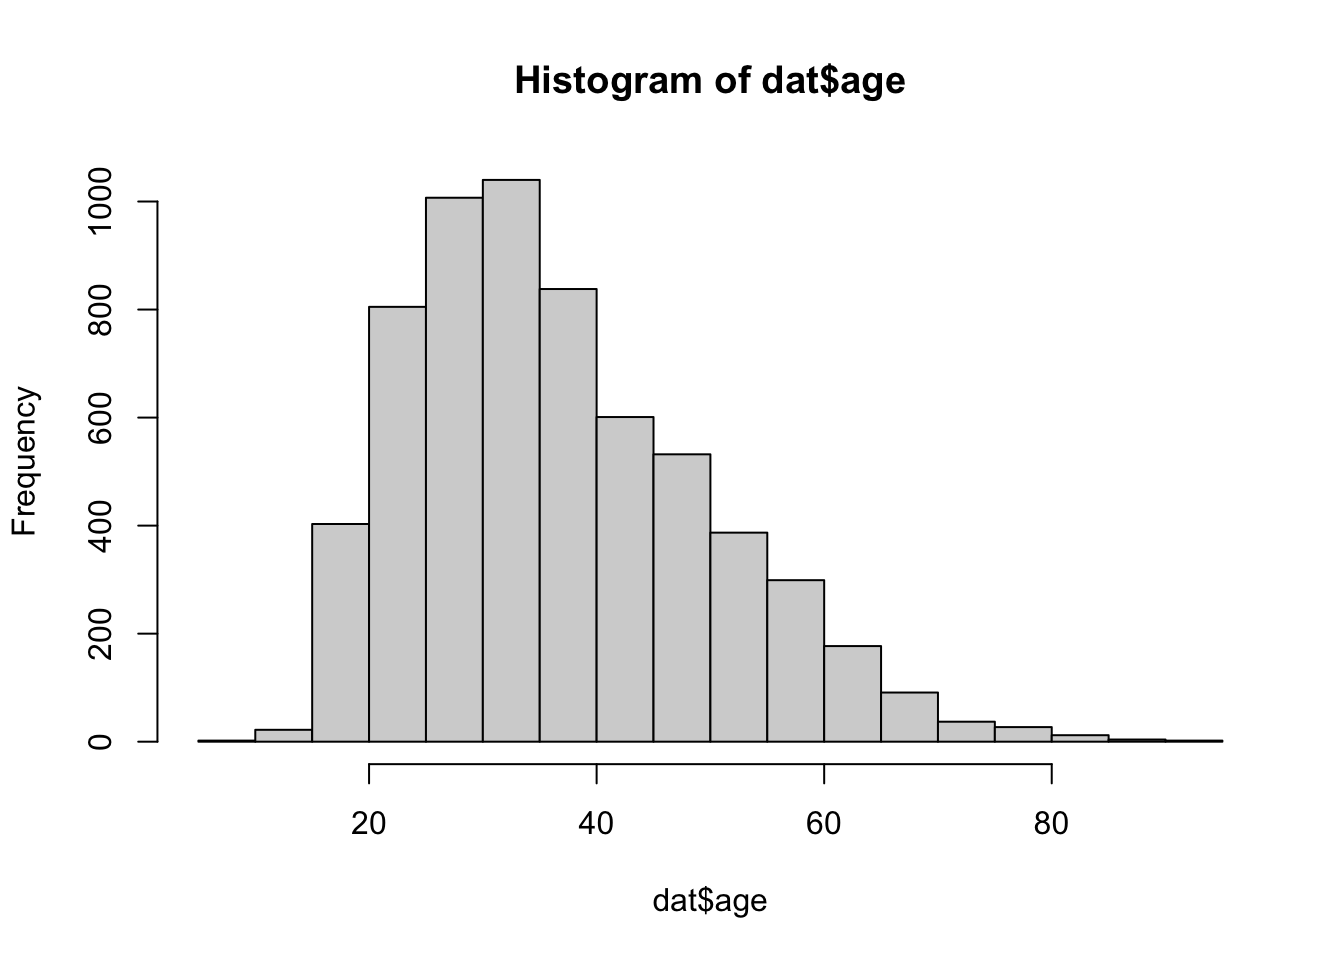
\includegraphics{Assignments_files/figure-latex/unnamed-chunk-25-1.pdf}

\textbf{The distribution shows a right skew to the ages of victims in
recorded fatal shootings. I feel like this is fairly predictable, as the
average age in the US is 38, and we know that fatal shootings often
occur in over-policed low-income areas where the majority of people who
are out and about are the working class of these areas, putting majority
of their ages around 20-40 years old.}

\begin{enumerate}
\def\labelenumi{\alph{enumi}.}
\setcounter{enumi}{1}
\tightlist
\item
  To understand the center of the age distribution, would you use a mean
  or a median, and why? Find the one you picked.
\end{enumerate}

\begin{Shaded}
\begin{Highlighting}[]
\FunctionTok{summary}\NormalTok{(dat}\SpecialCharTok{$}\NormalTok{age)}
\end{Highlighting}
\end{Shaded}

\begin{verbatim}
##    Min. 1st Qu.  Median    Mean 3rd Qu.    Max.    NA's 
##    6.00   27.00   35.00   37.12   45.00   91.00     308
\end{verbatim}

\textbf{I would use the median of the data. Because the data is skewed,
the median is a better measure of central tendency than the mean as it
is more representative of the sample given what we know about it's
distribution. The median is 35, as in 35 years old is the average age of
someone involved in a fatal shooting in the United States at the hand of
police.}

\begin{enumerate}
\def\labelenumi{\alph{enumi}.}
\setcounter{enumi}{2}
\tightlist
\item
  Describe the gender distribution of the sample. Do you find this
  surprising?
\end{enumerate}

\begin{Shaded}
\begin{Highlighting}[]
\FunctionTok{table}\NormalTok{(dat}\SpecialCharTok{$}\NormalTok{gender)}
\end{Highlighting}
\end{Shaded}

\begin{verbatim}
## 
##         F    M 
##    3  293 6298
\end{verbatim}

\textbf{I do find this surprising. Given that there is a fairly
predictable distribution of ages in this data set, you would assume
there be an equally as predictable distribution of gender. However,
knowing what we know about fatal shootings by police in the United
States, the narrative portrayed by police officers often follows the
line of not-being-confident-in-a-lack-of-threat-from-the-victim. While
this narrative is incredibly frustrating, it does align with the uneven
distribution of men and women in this event because women often are
portrayed as being a lower threat level than men in general.}

\hypertarget{problem-3-10-points}{%
\subsection{Problem 3 (10 points)}\label{problem-3-10-points}}

\begin{enumerate}
\def\labelenumi{\alph{enumi}.}
\tightlist
\item
  How many police officers had a body camera, according to news reports?
  What proportion is this of all the incidents in the data? Are you
  surprised that it is so high or low?
\end{enumerate}

\begin{Shaded}
\begin{Highlighting}[]
\FunctionTok{table}\NormalTok{(dat}\SpecialCharTok{$}\NormalTok{body\_camera)}
\end{Highlighting}
\end{Shaded}

\begin{verbatim}
## 
## False  True 
##  5684   910
\end{verbatim}

\begin{Shaded}
\begin{Highlighting}[]
\DecValTok{910}\SpecialCharTok{/}\DecValTok{6594}
\end{Highlighting}
\end{Shaded}

\begin{verbatim}
## [1] 0.1380042
\end{verbatim}

\begin{Shaded}
\begin{Highlighting}[]
\CommentTok{\# prop.table(dat$body\_camera)}
\CommentTok{\# would have to convert to numeric, can just get proportion via simple math}
\end{Highlighting}
\end{Shaded}

\textbf{According to the news, 910 of the officers had a body camera at
the time of the incident. This is 13.800\% of the incidents in this
data. This proportion being so low is surprising to me because I thought
that it was protocol as of the past few years for officers to wear body
cameras when on duty. The fact that this statistic is so low is very
concerning.}

\begin{enumerate}
\def\labelenumi{\alph{enumi}.}
\setcounter{enumi}{1}
\tightlist
\item
  In how many of the incidents was the victim fleeing? What proportion
  is this of the total number of incidents in the data? Is this what you
  would expect?
\end{enumerate}

\begin{Shaded}
\begin{Highlighting}[]
\FunctionTok{table}\NormalTok{(dat}\SpecialCharTok{$}\NormalTok{flee)}
\end{Highlighting}
\end{Shaded}

\begin{verbatim}
## 
##                     Car        Foot Not fleeing       Other 
##         491        1058         845        3952         248
\end{verbatim}

\begin{Shaded}
\begin{Highlighting}[]
\DecValTok{1058} \SpecialCharTok{+} \DecValTok{845}
\end{Highlighting}
\end{Shaded}

\begin{verbatim}
## [1] 1903
\end{verbatim}

\begin{Shaded}
\begin{Highlighting}[]
\DecValTok{1903}\SpecialCharTok{/}\DecValTok{6594}
\end{Highlighting}
\end{Shaded}

\begin{verbatim}
## [1] 0.2885957
\end{verbatim}

\textbf{The victim was fleeing in 1058 of the incidents (either by car
or on foot: ``other'' answers and not included answers on this were
excluded due to lack of information). This is 28.860\% of the data set.
This is not surprising given what we know about police brutality in the
United States, but it is very concerning. This means that over 70\% of
victims who were shot fatally by police were not fleeing.}

\hypertarget{problem-4-10-points---answer-only-one-of-these-a-or-b.}{%
\subsection{Problem 4 (10 points) - Answer only one of these (a or
b).}\label{problem-4-10-points---answer-only-one-of-these-a-or-b.}}

\begin{enumerate}
\def\labelenumi{\alph{enumi}.}
\tightlist
\item
  Describe the relationship between the variables ``body camera'' and
  ``flee'' using a stacked barplot. What can you conclude from this
  relationship?
\end{enumerate}

\emph{Hint 1: The categories along the x-axis are the options for
``flee'', each bar contains information about whether the police officer
had a body camera (vertically), and the height along the y-axis shows
the frequency of that category).}

\emph{Hint 2: Also, if you are unsure about the syntax for barplot, run
?barplot in R and see some examples at the bottom of the documentation.
This is usually a good way to look up the syntax of R code. You can also
Google it.}

\begin{Shaded}
\begin{Highlighting}[]
\NormalTok{counts }\OtherTok{\textless{}{-}} \FunctionTok{table}\NormalTok{(dat}\SpecialCharTok{$}\NormalTok{body\_camera, dat}\SpecialCharTok{$}\NormalTok{flee)}
\FunctionTok{barplot}\NormalTok{(counts, }\AttributeTok{col=}\FunctionTok{c}\NormalTok{(}\StringTok{"red"}\NormalTok{, }\StringTok{"blue"}\NormalTok{), }\AttributeTok{legend=}\ConstantTok{TRUE}\NormalTok{, }\AttributeTok{xlab=}\StringTok{"Flee"}\NormalTok{, }\AttributeTok{ylab=}\StringTok{"Frequency"}\NormalTok{)}
\end{Highlighting}
\end{Shaded}

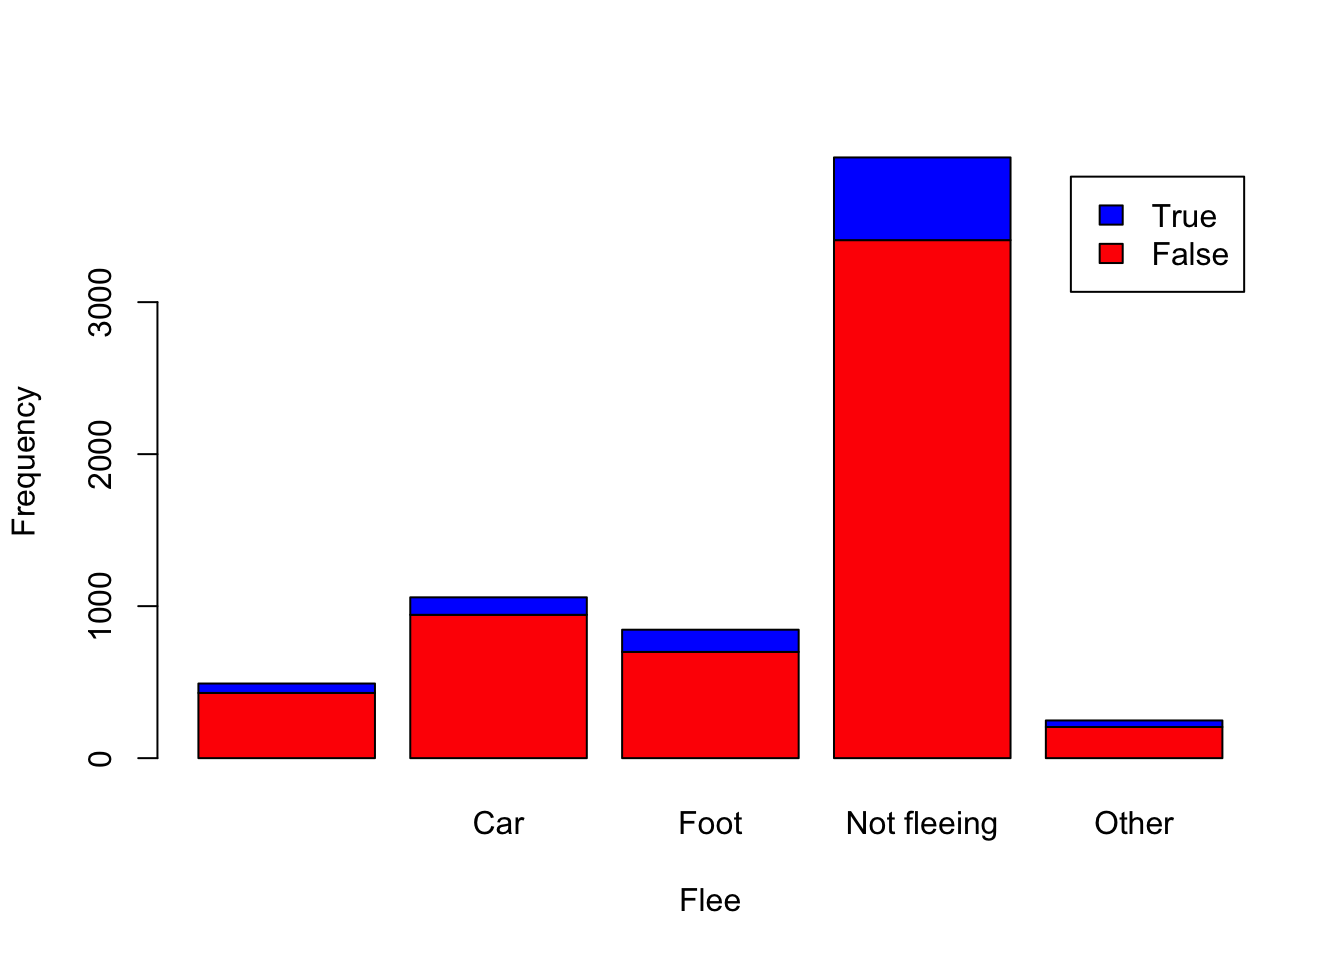
\includegraphics{Assignments_files/figure-latex/unnamed-chunk-30-1.pdf}

\textbf{From this relationship, we can see that there is an even
proportion of body cam presence across all flee categories,
demonstrating that the presence of a body cam does not seem to affect
whether or not someone in this study fled or not. Though there is a
section in the distribution that is unlabelled due to the flee variable
being unmarked in these instances, even this variable demonstrates an
even distribution.}

\begin{enumerate}
\def\labelenumi{\alph{enumi}.}
\setcounter{enumi}{1}
\tightlist
\item
  Describe the relationship between age and race by using a boxplot.
  What can you conclude from this relationship?
\end{enumerate}

\emph{Hint 1: The categories along the x-axis are the race categories
and the height along the y-axis is age.}

\emph{Hint 2: Also, if you are unsure about the syntax for boxplot, run
?boxplot in R and see some examples at the bottom of the documentation.
This is usually a good way to look up the syntax of R code. You can also
Google it.}

\textbf{Your answer here.}

\hypertarget{extra-credit-10-points}{%
\subsection{Extra credit (10 points)}\label{extra-credit-10-points}}

\begin{enumerate}
\def\labelenumi{\alph{enumi}.}
\tightlist
\item
  What does this code tell us?
\end{enumerate}

\begin{Shaded}
\begin{Highlighting}[]
\NormalTok{mydates }\OtherTok{\textless{}{-}} \FunctionTok{as.Date}\NormalTok{(dat}\SpecialCharTok{$}\NormalTok{date)}
\FunctionTok{head}\NormalTok{(mydates)}
\NormalTok{(mydates[}\FunctionTok{length}\NormalTok{(mydates)] }\SpecialCharTok{{-}}\NormalTok{ mydates[}\DecValTok{1}\NormalTok{])}
\end{Highlighting}
\end{Shaded}

\textbf{This code tells us the difference in time between the first and
last recorded date in the data set.}

\begin{enumerate}
\def\labelenumi{\alph{enumi}.}
\setcounter{enumi}{1}
\tightlist
\item
  On Friday, a new report was published that was described as follows by
  The Guardian: ``More than half of US police killings are mislabelled
  or not reported, study finds.'' Without reading this article now (due
  to limited time), why do you think police killings might be
  mislabelled or underreported?
\end{enumerate}

\textbf{Unfortunately, the reach of the police department is seen in the
representation of police killings in reportings. Because an accurate
report of fatal shootings at the hands of police relies on a pure and
fully not corrupted police force and governmental power, there would be
several levels of responsibility that would have to be upheld to ensure
that all incidents of fatal shootings by police would be reported
accurately. As the article by The Guardian says, ``The same government
responsible for this violence is also responsible for reporting on
it.''}

\begin{enumerate}
\def\labelenumi{\alph{enumi}.}
\setcounter{enumi}{2}
\tightlist
\item
  Regarding missing values in problem 4, do you see any? If so, do you
  think that's all that's missing from the data?
\end{enumerate}

\textbf{There is visibly missing data in the flee variable. This is
likely not all the data that is missing from the data set because it is
not rare for data to be missing in such a large data set like this.}

\hypertarget{assignment-3}{%
\section{Assignment 3}\label{assignment-3}}

This assignment is due on Canvas on Wednesday 10/27/2021 before class,
at 10:15 am. Include the name of anyone with whom you collaborated at
the top of the assignment.

Submit your responses as either an HTML file or a PDF file on Canvas.
Also, please upload it to your website.

Save the file (found on Canvas) crime\_simple.txt to the same folder as
this file (your Rmd file for Assignment 3).

Load the data.

\begin{Shaded}
\begin{Highlighting}[]
\FunctionTok{library}\NormalTok{(readr)}
\FunctionTok{library}\NormalTok{(knitr)}
\NormalTok{dat.crime }\OtherTok{\textless{}{-}} \FunctionTok{read\_delim}\NormalTok{(}\StringTok{"crime\_simple.txt"}\NormalTok{, }\AttributeTok{delim =} \StringTok{"}\SpecialCharTok{\textbackslash{}t}\StringTok{"}\NormalTok{)}
\end{Highlighting}
\end{Shaded}

\begin{verbatim}
## Rows: 47 Columns: 14
\end{verbatim}

\begin{verbatim}
## -- Column specification --------------------------------------------------------
## Delimiter: "\t"
## dbl (14): R, Age, S, Ed, Ex0, Ex1, LF, M, N, NW, U1, U2, W, X
\end{verbatim}

\begin{verbatim}
## 
## i Use `spec()` to retrieve the full column specification for this data.
## i Specify the column types or set `show_col_types = FALSE` to quiet this message.
\end{verbatim}

This is a dataset from a textbook by Brian S. Everitt about crime in the
US in 1960. The data originate from the Uniform Crime Report of the FBI
and other government sources. The data for 47 states of the USA are
given.

Here is the codebook:

R: Crime rate: \# of offenses reported to police per million population

Age: The number of males of age 14-24 per 1000 population

S: Indicator variable for Southern states (0 = No, 1 = Yes)

Ed: Mean of years of schooling x 10 for persons of age 25 or older

Ex0: 1960 per capita expenditure on police by state and local government

Ex1: 1959 per capita expenditure on police by state and local government

LF: Labor force participation rate per 1000 civilian urban males age
14-24

M: The number of males per 1000 females

N: State population size in hundred thousands

NW: The number of non-whites per 1000 population

U1: Unemployment rate of urban males per 1000 of age 14-24

U2: Unemployment rate of urban males per 1000 of age 35-39

W: Median value of transferable goods and assets or family income in
tens of \$

X: The number of families per 1000 earning below 1/2 the median income

We are interested in checking whether the reported crime rate (\# of
offenses reported to police per million population) and the average
education (mean number of years of schooling for persons of age 25 or
older) are related.

\begin{enumerate}
\def\labelenumi{\arabic{enumi}.}
\tightlist
\item
  How many observations are there in the dataset? To what does each
  observation correspond?
\end{enumerate}

\begin{Shaded}
\begin{Highlighting}[]
\FunctionTok{library}\NormalTok{(dplyr)}
\FunctionTok{count}\NormalTok{(dat.crime)}
\end{Highlighting}
\end{Shaded}

\begin{verbatim}
## # A tibble: 1 x 1
##       n
##   <int>
## 1    47
\end{verbatim}

\textbf{There are 47 observations in the dataset. The observations
correspond to the different rows, aka different states.}

\begin{enumerate}
\def\labelenumi{\arabic{enumi}.}
\setcounter{enumi}{1}
\tightlist
\item
  Draw a scatterplot of the two variables. Calculate the correlation
  between the two variables. Can you come up with an explanation for
  this relationship?
\end{enumerate}

\begin{Shaded}
\begin{Highlighting}[]
\FunctionTok{library}\NormalTok{(datasets)}
\FunctionTok{plot}\NormalTok{(dat.crime}\SpecialCharTok{$}\NormalTok{Ed,dat.crime}\SpecialCharTok{$}\NormalTok{R,  }\AttributeTok{main=}\StringTok{"Relationship between Reported Crime Rate and Average Education for 47 States"}\NormalTok{,}
    \AttributeTok{xlab=}\StringTok{"Average Education (mean number of years of schooling for persons of age 25 or older)"}\NormalTok{, }\AttributeTok{ylab=}\StringTok{"Crime Rate (\# of offenses reported to police per million population)"}\NormalTok{)}
\end{Highlighting}
\end{Shaded}

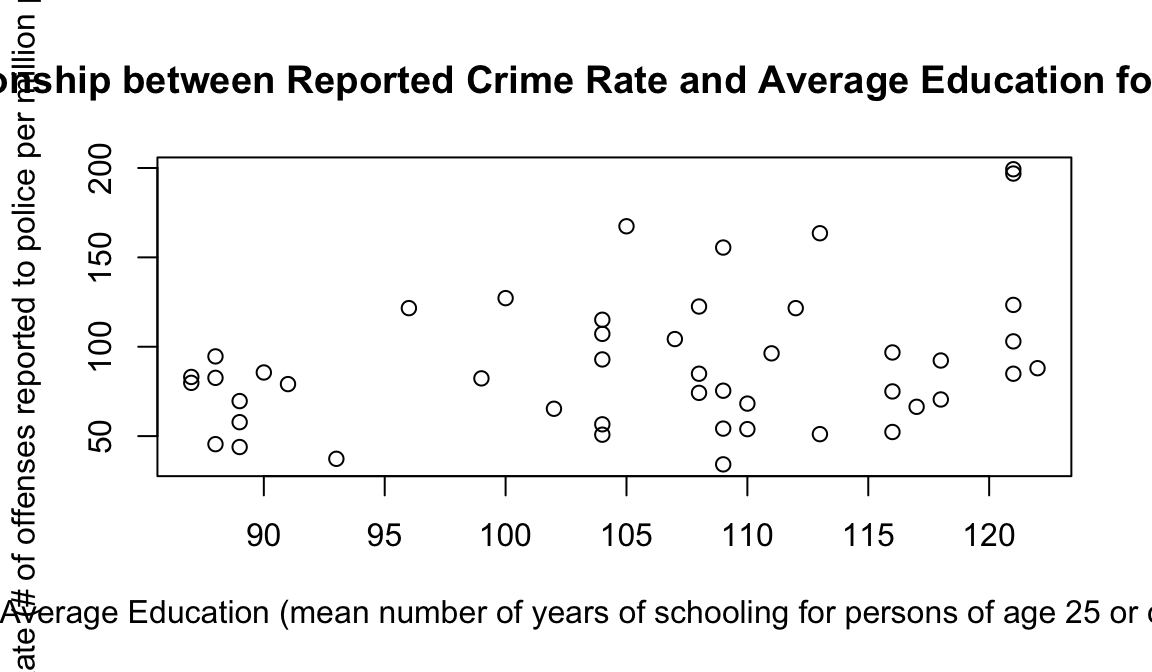
\includegraphics{Assignments_files/figure-latex/unnamed-chunk-35-1.pdf}

\begin{Shaded}
\begin{Highlighting}[]
\NormalTok{x }\OtherTok{\textless{}{-}} \FunctionTok{cor}\NormalTok{(dat.crime}\SpecialCharTok{$}\NormalTok{R, dat.crime}\SpecialCharTok{$}\NormalTok{Ed)}
\NormalTok{x}
\end{Highlighting}
\end{Shaded}

\begin{verbatim}
## [1] 0.3228349
\end{verbatim}

\textbf{I cannot come up with an explanation for this relationship on
first impression. The correlation of these two variables is 0.3228349,
meaning that there is a fairly weak correlation. Because there are so
many other factors in this dataset, we can assume that there is likely
another factor that correlates more highly to the reported crime rate,
but this low of a correlation does not allow us to make any causal
inferences.}

\begin{enumerate}
\def\labelenumi{\arabic{enumi}.}
\setcounter{enumi}{2}
\tightlist
\item
  Regress reported crime rate (y) on average education (x) and call this
  linear model \texttt{crime.lm} and write the summary of the regression
  by using this code, which makes it look a little nicer
  \texttt{\{r,\ eval=FALSE\}\ kable(summary(crime.lm)\$coef,\ digits\ =\ 2)}.
\end{enumerate}

\begin{Shaded}
\begin{Highlighting}[]
\CommentTok{\# Remember to remove eval=FALSE above!}

\NormalTok{dat.crime}\SpecialCharTok{$}\NormalTok{R.c }\OtherTok{=} \FunctionTok{scale}\NormalTok{(dat.crime}\SpecialCharTok{$}\NormalTok{R, }\AttributeTok{center=}\ConstantTok{TRUE}\NormalTok{, }\AttributeTok{scale=}\ConstantTok{FALSE}\NormalTok{)}
\NormalTok{crime.lm }\OtherTok{\textless{}{-}} \FunctionTok{lm}\NormalTok{(}\AttributeTok{formula =}\NormalTok{ Ed }\SpecialCharTok{\textasciitilde{}}\NormalTok{ R.c, }\AttributeTok{data =}\NormalTok{ dat.crime) }
\FunctionTok{kable}\NormalTok{(}\FunctionTok{summary}\NormalTok{(crime.lm)}\SpecialCharTok{$}\NormalTok{coef, }\AttributeTok{digits =} \DecValTok{2}\NormalTok{)}
\end{Highlighting}
\end{Shaded}

\begin{longtable}[]{@{}lrrrr@{}}
\toprule
& Estimate & Std. Error & t value &
Pr(\textgreater\textbar t\textbar) \\
\midrule
\endhead
(Intercept) & 105.64 & 1.56 & 67.65 & 0.00 \\
R.c & 0.09 & 0.04 & 2.29 & 0.03 \\
\bottomrule
\end{longtable}

\begin{Shaded}
\begin{Highlighting}[]
\FunctionTok{summary}\NormalTok{(crime.lm)}
\end{Highlighting}
\end{Shaded}

\begin{verbatim}
## 
## Call:
## lm(formula = Ed ~ R.c, data = dat.crime)
## 
## Residuals:
##     Min      1Q  Median      3Q     Max 
## -18.020  -8.441   1.528   8.200  16.596 
## 
## Coefficients:
##              Estimate Std. Error t value Pr(>|t|)    
## (Intercept) 105.63830    1.56148  67.653   <2e-16 ***
## R.c           0.09338    0.04081   2.288   0.0269 *  
## ---
## Signif. codes:  0 '***' 0.001 '**' 0.01 '*' 0.05 '.' 0.1 ' ' 1
## 
## Residual standard error: 10.7 on 45 degrees of freedom
## Multiple R-squared:  0.1042, Adjusted R-squared:  0.08432 
## F-statistic: 5.236 on 1 and 45 DF,  p-value: 0.02688
\end{verbatim}

\begin{enumerate}
\def\labelenumi{\arabic{enumi}.}
\setcounter{enumi}{3}
\tightlist
\item
  Are the four assumptions of linear regression satisfied? To answer
  this, draw the relevant plots. (Write a maximum of one sentence per
  assumption.)
\end{enumerate}

\begin{Shaded}
\begin{Highlighting}[]
\CommentTok{\# plot 1 \& plot 2, residuals vs x}
\FunctionTok{plot}\NormalTok{(dat.crime}\SpecialCharTok{$}\NormalTok{R.c, crime.lm}\SpecialCharTok{$}\NormalTok{residuals, }\AttributeTok{ylim=}\FunctionTok{c}\NormalTok{(}\SpecialCharTok{{-}}\DecValTok{15}\NormalTok{,}\DecValTok{15}\NormalTok{), }\AttributeTok{main=}\StringTok{"Residuals vs. x"}\NormalTok{, }\AttributeTok{xlab=}\StringTok{"x, Scaled Crime Rates"}\NormalTok{, }\AttributeTok{ylab=}\StringTok{"Residuals"}\NormalTok{)}
\FunctionTok{abline}\NormalTok{(}\AttributeTok{h =} \DecValTok{0}\NormalTok{, }\AttributeTok{lty=}\StringTok{"dashed"}\NormalTok{)}
\end{Highlighting}
\end{Shaded}

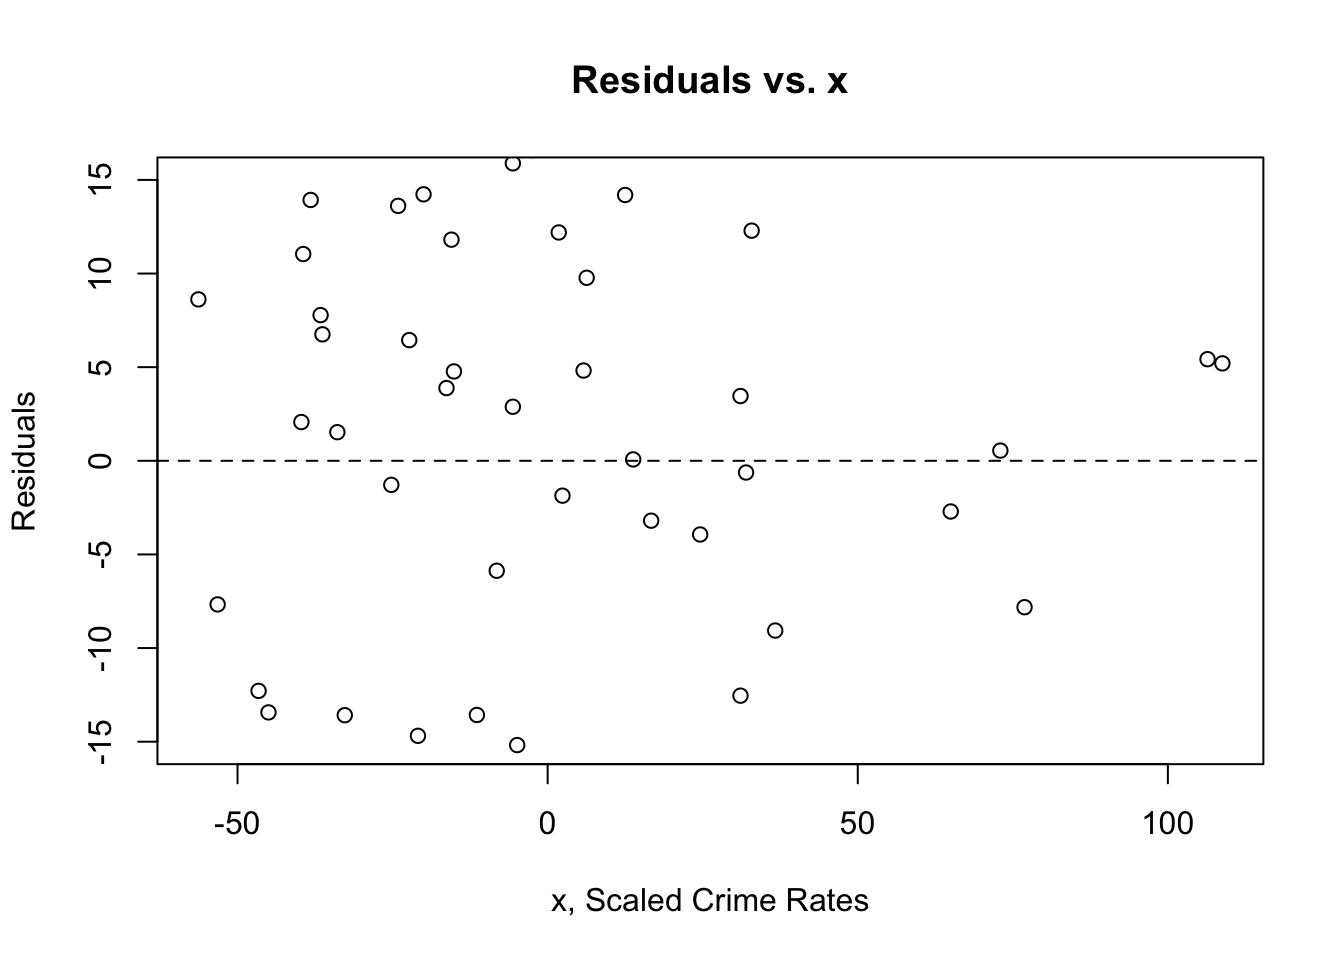
\includegraphics{Assignments_files/figure-latex/unnamed-chunk-37-1.pdf}

\begin{Shaded}
\begin{Highlighting}[]
\CommentTok{\# plot 3}
\FunctionTok{plot}\NormalTok{(crime.lm, }\AttributeTok{which=}\DecValTok{3}\NormalTok{)}
\end{Highlighting}
\end{Shaded}

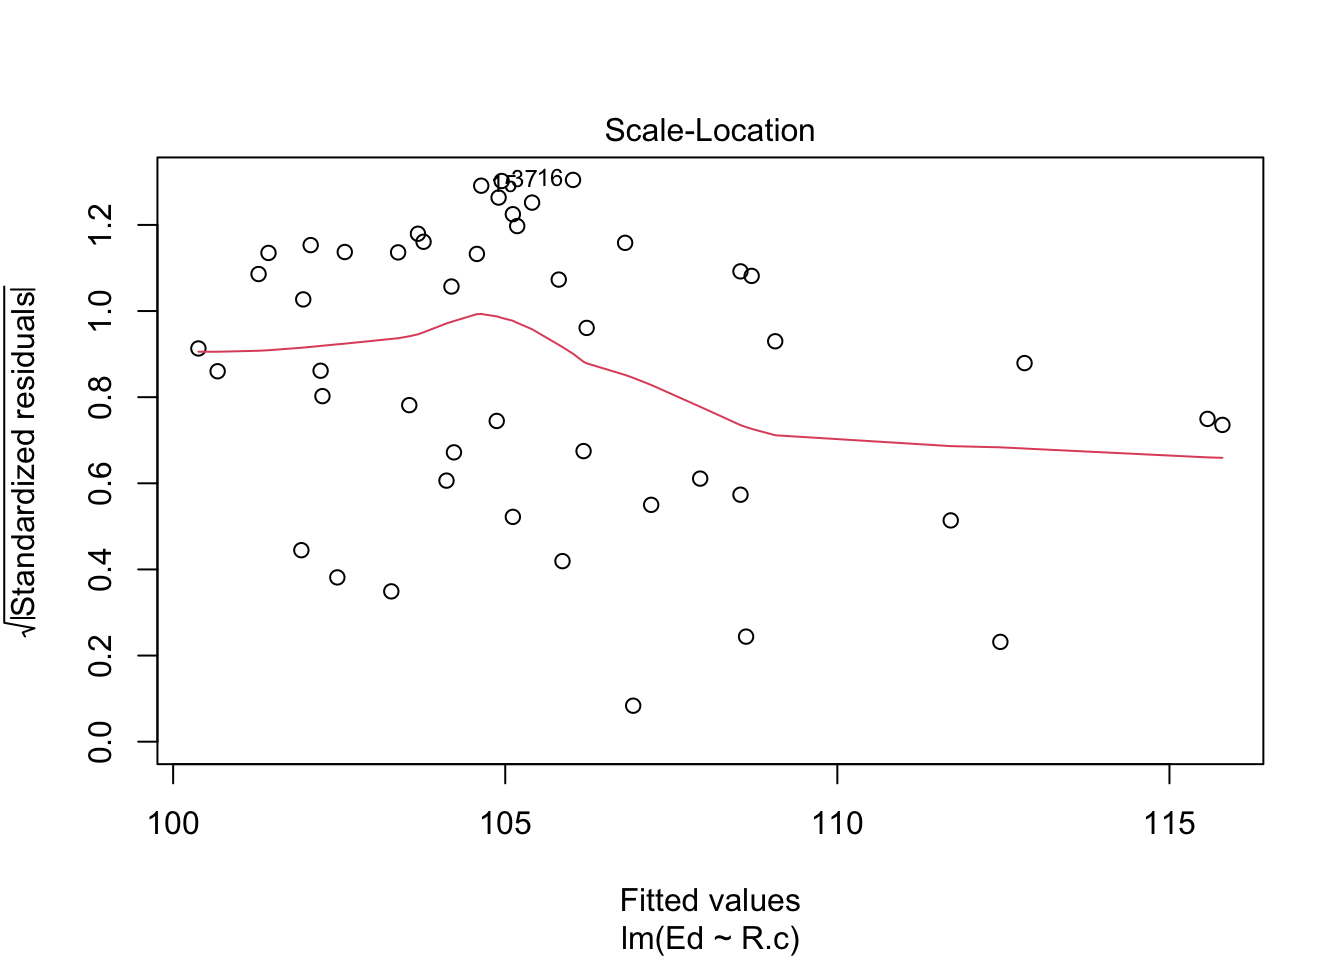
\includegraphics{Assignments_files/figure-latex/unnamed-chunk-37-2.pdf}

\begin{Shaded}
\begin{Highlighting}[]
\CommentTok{\# plot 4, qq and outlier condition}
\FunctionTok{plot}\NormalTok{(crime.lm, }\AttributeTok{which=}\DecValTok{2}\NormalTok{)}
\end{Highlighting}
\end{Shaded}

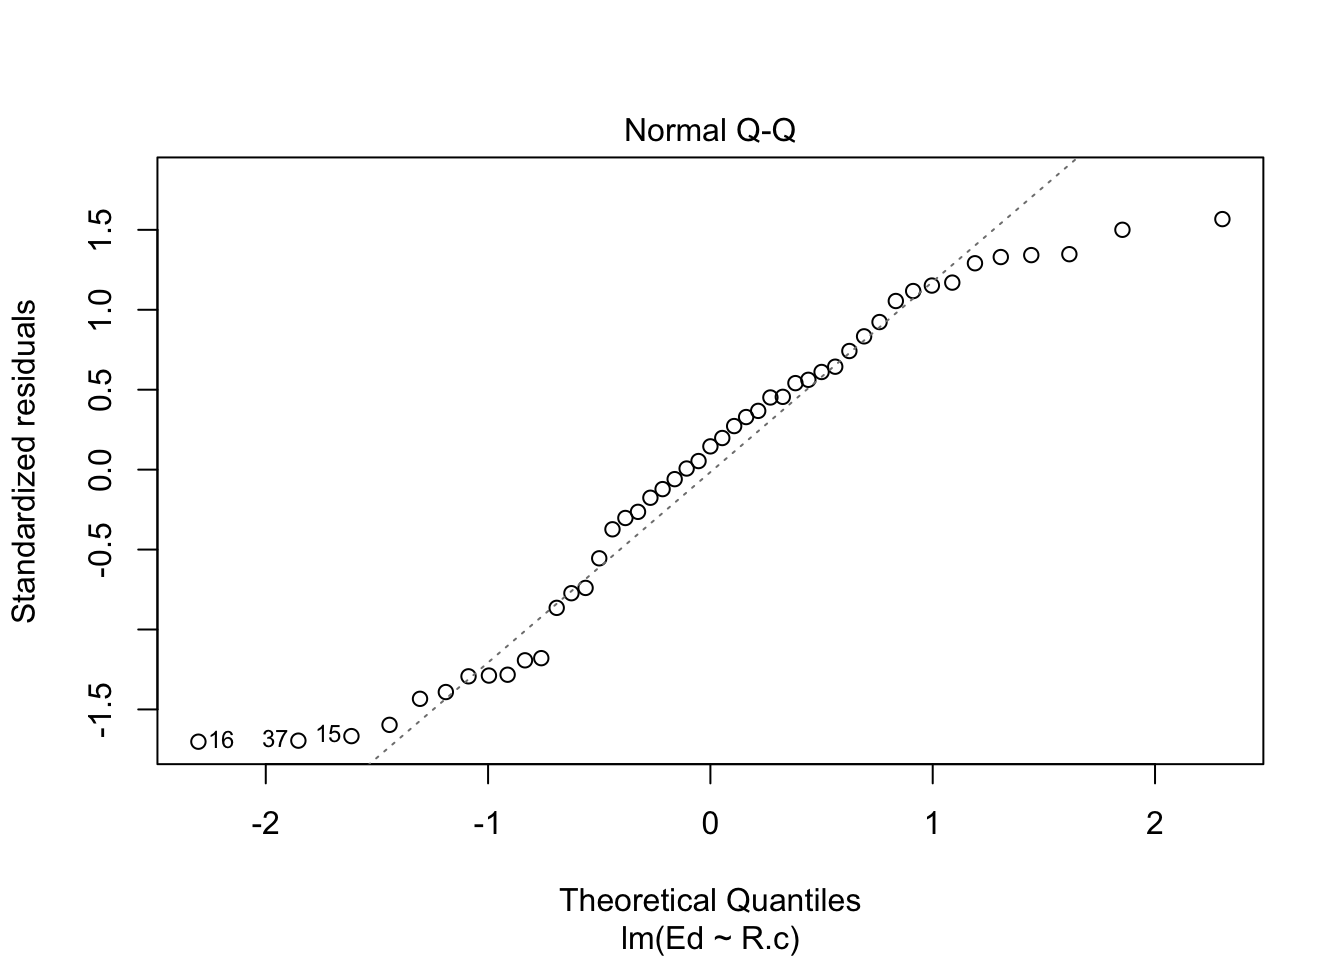
\includegraphics{Assignments_files/figure-latex/unnamed-chunk-37-3.pdf}

\begin{Shaded}
\begin{Highlighting}[]
\FunctionTok{plot}\NormalTok{(crime.lm, }\AttributeTok{which=}\DecValTok{5}\NormalTok{)}
\end{Highlighting}
\end{Shaded}

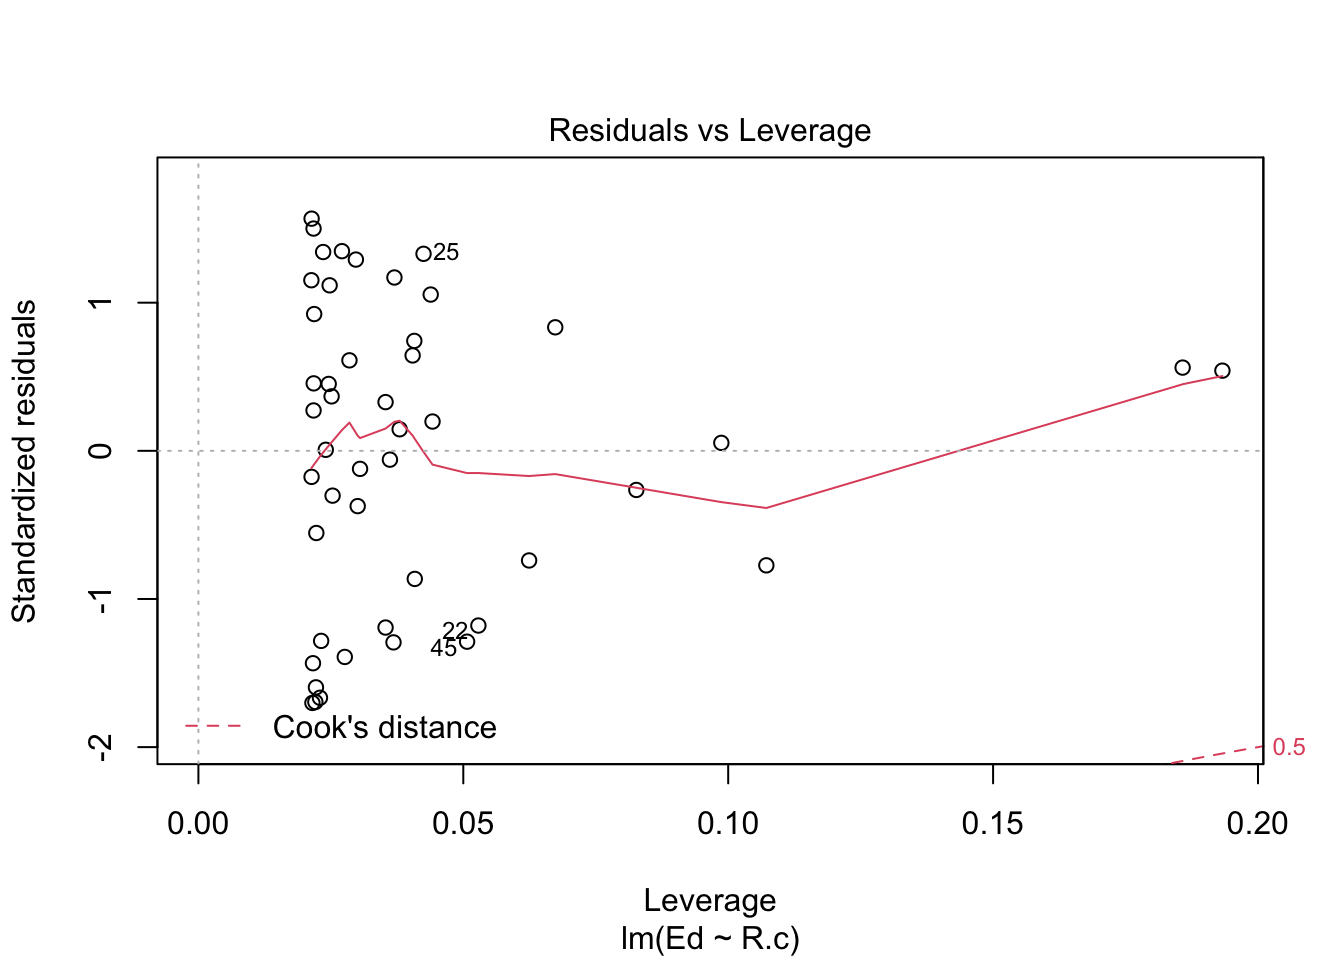
\includegraphics{Assignments_files/figure-latex/unnamed-chunk-37-4.pdf}

\textbf{The four assumptions are as follows: linearity, independence,
equal variance, and normal population. The first assumption - linearity
- is not satisfied because the first plot of the residuals vs x does not
have a horizontal direction. The second assumption - independence - is
satisfied because the plot of residuals vs x does not display any
distinct patterns. The third assumption - equal variance - is satisfied
because the flat line shows that the errors are of constant variance.
The fourth assumption - normal population - is not satisfied because the
qq plot is heavily tailed, meaning it does not follow the normal model
well.}

\begin{enumerate}
\def\labelenumi{\arabic{enumi}.}
\setcounter{enumi}{4}
\tightlist
\item
  Is the relationship between reported crime and average education
  statistically significant? Report the estimated coefficient of the
  slope, the standard error, and the p-value. What does it mean for the
  relationship to be statistically significant?
\end{enumerate}

\textbf{The estimated coefficient is 0.09. The standard error is 0.04.
The p-value is 0.02688. This means that this relationship is
statistically significant, as the p-value is less than 0.05. If the
relationship is statistically significant, this means that there is a
high likelihood that the observance is not wrong or random (I use this
word carefully) chance.}

\begin{enumerate}
\def\labelenumi{\arabic{enumi}.}
\setcounter{enumi}{5}
\tightlist
\item
  How are reported crime and average education related? In other words,
  for every unit increase in average education, how does reported crime
  rate change (per million) per state?
\end{enumerate}

\textbf{For every unit increase in average education, the reported crime
rate increases by 0.09 units, meaning that the reported crime rate
increases by 0.09 offenses reported to police per million population.}

\begin{enumerate}
\def\labelenumi{\arabic{enumi}.}
\setcounter{enumi}{6}
\tightlist
\item
  Can you conclude that if individuals were to receive more education,
  then crime will be reported more often? Why or why not?
\end{enumerate}

\textbf{We cannot conclude this from the dataset. While it appears there
is a statistically significant correlation, this does not mean we can
assume causation. While the variables correlate to each other, this is
not conducive of a causal relationship.}

\hypertarget{assignment-4}{%
\section{Assignment 4}\label{assignment-4}}

\hypertarget{pt-1}{%
\subsection{3 (pt 1)}\label{pt-1}}

\hypertarget{loading-the-library-of-tidyverse-where-the-tidyverse-package-is-stored-to-access}{%
\paragraph{loading the library of tidyverse where the tidyverse package
is stored to
access}\label{loading-the-library-of-tidyverse-where-the-tidyverse-package-is-stored-to-access}}

\hypertarget{ggplot}{%
\paragraph{ggplot}\label{ggplot}}

library(tidyverse) \#installing the package so one can reload it after
every session install.packages(``tidyverse'') \#\#\#\# calling mpg
dataframe A data frame is a rectangular collection of variables (in the
columns) and observations (in the rows). mpg contains observations
collected by the US Environmental Protection Agency on 38 models of
cars. \#\#\#\# mapping a gg scatterplot that maps car's engine size
against fuel efficiency \#\#\#\# shwos a negative relationship between x
and y variables ggplot(data = mpg) + geom\_point(mapping = aes(x =
displ, y = hwy)) \#\#\#\# creating a reusable template for making graphs
with ggplot2 ggplot(data = ) + (mapping = aes()) \#\#\#\# mapping
aesthetics in your plot to the variables in the dataset, maps class to
\#\#\#\# color aesthetic ggplot(data = mpg) + geom\_point(mapping =
aes(x = displ, y = hwy, color = class)) \#\#\#\# mapping class against
size aesthetic ggplot(data = mpg) + geom\_point(mapping = aes(x = displ,
y = hwy, size = class)) \#\#\#\# mapping class to the alpha aesthetic,
which controls the transparency of the points, or to the shape
aesthetic, which controls the shape of the points \#\#\#\# left
ggplot(data = mpg) + geom\_point(mapping = aes(x = displ, y = hwy, alpha
= class)) \#\#\#\# right ggplot(data = mpg) + geom\_point(mapping =
aes(x = displ, y = hwy, shape = class)) \#\#\#\# setting aesthetic
properties of geom manually, making all of the points blue ggplot(data =
mpg) + geom\_point(mapping = aes(x = displ, y = hwy), color = ``blue'')
\#\#\#\# missed parentheses so the point do not come out blue
ggplot(data = mpg) + geom\_point(mapping = aes(x = displ, y = hwy, color
= ``blue'')) \#\#\#\# plus sign must come at the end of the line not the
beginning ggplot(data = mpg) + geom\_point(mapping = aes(x = displ, y =
hwy)) \#\#\#\# facetting plot by a single variable. First argument is a
formula, followed by \textasciitilde{} \# followed by variable name
where formula is the name of a data structure in R/ The variable that
\#\#\#\# is passed to facet\_wrap should be discrete ggplot(data = mpg)
+ geom\_point(mapping = aes(x = displ, y = hwy)) +
facet\_wrap(\textasciitilde{} class, nrow = 2) \#\#\#\# Facetting your
plot on the combination of two variables, add facet\_grid() to your plot
call. The first argument of facet\_grid() is also a formula. This time
the formula should contain two variable names separated by a
\textasciitilde. The empty grids show that there is no data attributed
to this specific variable ggplot(data = mpg) + geom\_point(mapping =
aes(x = displ, y = hwy)) + facet\_grid(drv \textasciitilde{} cyl)
\#\#\#\# Code creates 4 facet columns that are generated by the ``.''
The data maps engine size against fuel efficiency ggplot(data = mpg) +
geom\_point(mapping = aes(x = displ, y = hwy)) + facet\_grid(drv
\textasciitilde{} .) ggplot(data = mpg) + geom\_point(mapping = aes(x =
displ, y = hwy)) + facet\_grid(. \textasciitilde{} cyl) \#\#\#\# facets
columns and rows of each type of car variable, engine size against fuel
efficiency ggplot(data = mpg) + geom\_point(mapping = aes(x = displ, y =
hwy)) + facet\_wrap(\textasciitilde{} class, nrow = 2) \#\#\#\# point
geom representation of the data \#\#\#\# left ggplot(data = mpg) +
geom\_point(mapping = aes(x = displ, y = hwy)) \#\#\#\# right smooth
geom representation of the data ggplot(data = mpg) +
geom\_smooth(mapping = aes(x = displ, y = hwy)) \#\#\#\# drawing a
different line, with a different linetype, for each unique value of the
variable that you map to linetype. ggplot(data = mpg) +
geom\_smooth(mapping = aes(x = displ, y = hwy, linetype = drv)) \#\#\#\#
geom smooth uses a single geometric object to display multiple rows of
data. \#\#\#\# Setting the group aesthetic to a categorical variable to
draw multiple objects. \#\#\#\# ggplot2 draws a separate object for each
unique value of the grouping variable. \#\#\#\# In practice, ggplot2
will automatically group the data for these geoms whenever you map an
aesthetic to a discrete variable (linetype example) ggplot(data = mpg) +
geom\_smooth(mapping = aes(x = displ, y = hwy))

ggplot(data = mpg) + geom\_smooth(mapping = aes(x = displ, y = hwy,
group = drv))

ggplot(data = mpg) + geom\_smooth( mapping = aes(x = displ, y = hwy,
color = drv), show.legend = FALSE ) \#\#\#\# displaying multiple geoms
in the same plot by adding multiple geom functions to ggplot ggplot(data
= mpg) + geom\_point(mapping = aes(x = displ, y = hwy)) +
geom\_smooth(mapping = aes(x = displ, y = hwy)) \#\#\#\# Avoiding
duplication of variables by passing a set of mappings to ggplot()
ggplot(data = mpg, mapping = aes(x = displ, y = hwy)) + geom\_point() +
geom\_smooth() \#\#\#\# Placing mappings in a geom function, ggplot2
treats them as local mappings for the layer. Uses these mappings to
extend or overwrite the global mappings for that layer only. This makes
it possible to display different aesthetics in different layers.
ggplot(data = mpg, mapping = aes(x = displ, y = hwy)) +
geom\_point(mapping = aes(color = class)) + geom\_smooth() \#\#\#\#
smooth line displays just a subset of the mpg dataset, the subcompact
cars. \#\#\#\# local data argument in geom\_smooth() overrides the
global data argument in ggplot() for that layer only. ggplot(data = mpg,
mapping = aes(x = displ, y = hwy)) + geom\_point(mapping = aes(color =
class)) + geom\_smooth(data = filter(mpg, class == ``subcompact''), se =
FALSE) \#\#\#\# Point plot with smooth line mapping separated by color
ggplot(data = mpg, mapping = aes(x = displ, y = hwy, color = drv)) +
geom\_point() + geom\_smooth(se = FALSE) \#\#\#\# Same graph by avoiding
duplication of variables by passing in the mapping function ggplot(data
= mpg, mapping = aes(x = displ, y = hwy)) + geom\_point() +
geom\_smooth()

ggplot() + geom\_point(data = mpg, mapping = aes(x = displ, y = hwy)) +
geom\_smooth(data = mpg, mapping = aes(x = displ, y = hwy))
\#\#\#\#generates bar plot of the diamonds dataset showing that more
diamonds are available with high quality cuts than with low quality cuts
ggplot(data = diamonds) + geom\_bar(mapping = aes(x = cut)) \#\#\#\#
Using geoms and stats interchangeably. You can recreate the previous
plot using stat\_count() instead of geom\_bar() ggplot(data = diamonds)
+ stat\_count(mapping = aes(x = cut)) \#\#\#\# Overriding the default
stat. change the stat of geom\_bar() from count (the default) to
identity. Lets one map the height of the bars to the raw values of a y
variable demo \textless- tribble( \textasciitilde cut,
\textasciitilde freq, ``Fair'', 1610, ``Good'', 4906, ``Very Good'',
12082, ``Premium'', 13791, ``Ideal'', 21551 )

ggplot(data = demo) + geom\_bar(mapping = aes(x = cut, y = freq), stat =
``identity'') \#\#\#\# displaying a bar chart of proportion rather than
count ggplot(data = diamonds) + geom\_bar(mapping = aes(x = cut, y =
stat(prop), group = 1)) \#\#\#\# summarises the y values for each unique
x value, to draw attention to the summary that you're computing
ggplot(data = diamonds) + stat\_summary( mapping = aes(x = cut, y =
depth), fun.min = min, fun.max = max, fun = median ) \#\#\#\# creates
proportion bar chart that is color coordinated where proportion is = 1
because proportions cannot exceed 100\% ggplot(data = diamonds) +
geom\_bar(mapping = aes(x = cut, y = after\_stat(prop))) ggplot(data =
diamonds) + geom\_bar(mapping = aes(x = cut, fill = color, y =
after\_stat(prop))) \#\#\#\# Coloring bars using function colour and
fill ggplot(data = diamonds) + geom\_bar(mapping = aes(x = cut, colour =
cut)) ggplot(data = diamonds) + geom\_bar(mapping = aes(x = cut, fill =
cut)) \#\#\#\#map the fill aesthetic to another variable, like clarity:
the bars are automatically stacked. Each colored rectangle represents a
combination of cut and clarity ggplot(data = diamonds) +
geom\_bar(mapping = aes(x = cut, fill = clarity)) \#\#\#\# position =
``identity'' will place each object exactly where it falls in the
context of the graph. Makes them transparent for easier viewing
ggplot(data = diamonds, mapping = aes(x = cut, fill = clarity)) +
geom\_bar(alpha = 1/5, position = ``identity'') ggplot(data = diamonds,
mapping = aes(x = cut, colour = clarity)) + geom\_bar(fill = NA,
position = ``identity'') \#\#\#\# position = ``fill'' works like
stacking, but makes each set of stacked bars the same height.
ggplot(data = diamonds) + geom\_bar(mapping = aes(x = cut, fill =
clarity), position = ``fill'') \#\#\#\# position = ``dodge'' places
overlapping objects directly beside one another. ggplot(data = diamonds)
+ geom\_bar(mapping = aes(x = cut, fill = clarity), position =
``dodge'') \#\#\#\# position = ``jitter'' adds a small amount of random
noise to each point. This spreads the points out because no two points
are likely to receive the same amount of random noise. ggplot(data =
mpg) + geom\_point(mapping = aes(x = displ, y = hwy), position =
``jitter'') \#\#\#\# point plot that does not include jittering to add
random noise ggplot(data = mpg, mapping = aes(x = cty, y = hwy)) +
geom\_point() \#\#\#\# coord\_flip() switches the x and y axes. This is
useful (for example), if you want horizontal boxplots ggplot(data = mpg,
mapping = aes(x = class, y = hwy)) + geom\_boxplot() ggplot(data = mpg,
mapping = aes(x = class, y = hwy)) + geom\_boxplot() + coord\_flip()
\#\#\#\# oord\_quickmap() sets the aspect ratio correctly for maps. nz
\textless- map\_data(``nz'')

ggplot(nz, aes(long, lat, group = group)) + geom\_polygon(fill =
``white'', colour = ``black'')

ggplot(nz, aes(long, lat, group = group)) + geom\_polygon(fill =
``white'', colour = ``black'') + coord\_quickmap() \#\#\#\#
coord\_polar() uses polar coordinates. Polar coordinates reveal an
interesting connection between a bar chart and a Coxcomb chart bar
\textless- ggplot(data = diamonds) + geom\_bar( mapping = aes(x = cut,
fill = cut), show.legend = FALSE, width = 1 ) + theme(aspect.ratio = 1)
+ labs(x = NULL, y = NULL)

bar + coord\_flip() bar + coord\_polar() \#\#\#\# generates a regression
line for the plot - shows that there is not a good relationship between
the two variables. Creates a point plot without randomness ggplot(data =
mpg, mapping = aes(x = cty, y = hwy)) + geom\_point() + geom\_abline() +
coord\_fixed()

\hypertarget{pt-2}{%
\subsection{28 (pt 2)}\label{pt-2}}

library(tidyverse) \#\#\#\# this line is loading the package `tidyverse'
which we already have installed ggplot(mpg, aes(displ, hwy)) +
geom\_point(aes(color = class)) + geom\_smooth(se = FALSE) + labs(title
= ``Fuel efficiency generally decreases with engine size'') \#\#\#\#
this section is making a scatterplot with the function geom\_point and
then making a line of best fit using the geom\_smooth function \#\#\#\#
this section also employs the labs function to make the label for the
title of the graph ggplot(mpg, aes(displ, hwy)) + geom\_point(aes(color
= class)) + geom\_smooth(se = FALSE) + labs( title = ``Fuel efficiency
generally decreases with engine size'', subtitle = ``Two seaters (sports
cars) are an exception because of their light weight'', caption = ``Data
from fueleconomy.gov'' ) \#\#\#\# this section does the same as the last
- the only difference is that it uses the labs function to also add a
subtitle and caption to the graph ggplot(mpg, aes(displ, hwy)) +
geom\_point(aes(colour = class)) + geom\_smooth(se = FALSE) + labs( x =
``Engine displacement (L)'', y = ``Highway fuel economy (mpg)'', colour
= ``Car type'' ) \#\#\#\# this section does the same as the last - the
only difference is that it uses x and y to define the axes labels and
makes the legend label ``car type'' df \textless- tibble( x = runif(10),
y = runif(10) ) ggplot(df, aes(x, y)) + geom\_point() + labs( x =
quote(sum(x{[}i{]} \^{} 2, i == 1, n)), y = quote(alpha + beta +
frac(delta, theta)) ) \#\#\#\# this section is creating a data frame
using the tibble function \#\#\#\# it also uses mathematical functions
in place of strings for the axes using the quote function
best\_in\_class \textless- mpg \%\textgreater\% group\_by(class)
\%\textgreater\% filter(row\_number(desc(hwy)) == 1)

ggplot(mpg, aes(displ, hwy)) + geom\_point(aes(colour = class)) +
geom\_text(aes(label = model), data = best\_in\_class) \#\#\#\# this
section pulls out the highest rated of each class, in this case the most
efficient cars ggplot(mpg, aes(displ, hwy)) + geom\_point(aes(colour =
class)) + geom\_label(aes(label = model), data = best\_in\_class,
nudge\_y = 2, alpha = 0.5) \#\#\#\# this section uses the geom\_label
function to draw a rectangle behind the text, with nudge\_y moving the
labels above the corresponding points ggplot(mpg, aes(displ, hwy)) +
geom\_point(aes(colour = class)) + geom\_point(size = 3, shape = 1, data
= best\_in\_class) + ggrepel::geom\_label\_repel(aes(label = model),
data = best\_in\_class) \#\#\#\# this section uses the ggrepel package
to automatically adjust labels so they don't overlap class\_avg
\textless- mpg \%\textgreater\% group\_by(class) \%\textgreater\%
summarise( displ = median(displ), hwy = median(hwy) )

ggplot(mpg, aes(displ, hwy, colour = class)) +
ggrepel::geom\_label\_repel(aes(label = class), data = class\_avg, size
= 6, label.size = 0, segment.color = NA ) + geom\_point() +
theme(legend.position = ``none'') \#\#\#\# this section replaces the
legend with labels on the plot label \textless- mpg \%\textgreater\%
summarise( displ = max(displ), hwy = max(hwy), label = ``Increasing
engine size is \nrelated to decreasing fuel economy.'' )

ggplot(mpg, aes(displ, hwy)) + geom\_point() + geom\_text(aes(label =
label), data = label, vjust = ``top'', hjust = ``right'') \#\#\#\# this
section adds a single label to the plot by creating a new data frame
label \textless- tibble( displ = Inf, hwy = Inf, label = ``Increasing
engine size is \nrelated to decreasing fuel economy.'' )

ggplot(mpg, aes(displ, hwy)) + geom\_point() + geom\_text(aes(label =
label), data = label, vjust = ``top'', hjust = ``right'') \#\#\#\# this
section places the text we just created directly on the borders of the
plot ``Increasing engine size is related to decreasing fuel economy.''
\%\textgreater\% stringr::str\_wrap(width = 40) \%\textgreater\%
writeLines() \#\#\#\# this section adds line breaks given the number of
characters ggplot(mpg, aes(displ, hwy)) + geom\_point(aes(colour =
class)) + scale\_x\_continuous() + scale\_y\_continuous() +
scale\_colour\_discrete() \#\#\#\# this section chooses scales that are
not the default ggplot(mpg, aes(displ, hwy)) + geom\_point() +
scale\_y\_continuous(breaks = seq(15, 40, by = 5)) \#\#\#\# this section
uses the break function to override the default choice of axes ticks
ggplot(mpg, aes(displ, hwy)) + geom\_point() +
scale\_x\_continuous(labels = NULL) + scale\_y\_continuous(labels =
NULL) \#\#\#\# this section uses labels = NULL to get rid of the numeric
tick labels on the axes presidential \%\textgreater\% mutate(id = 33 +
row\_number()) \%\textgreater\% ggplot(aes(start, id)) + geom\_point() +
geom\_segment(aes(xend = end, yend = id)) + scale\_x\_date(NULL, breaks
= presidential\$start, date\_labels = ``'\%y'') \#\#\#\# this section
uses the breaks function to highlight the observations in the data set
base \textless- ggplot(mpg, aes(displ, hwy)) + geom\_point(aes(colour =
class))

base + theme(legend.position = ``left'') base + theme(legend.position =
``top'') base + theme(legend.position = ``bottom'') base +
theme(legend.position = ``right'') \# the default \#\#\#\# this section
controls where the legel is drawn ggplot(mpg, aes(displ, hwy)) +
geom\_point(aes(colour = class)) + geom\_smooth(se = FALSE) +
theme(legend.position = ``bottom'') + guides(colour = guide\_legend(nrow
= 1, override.aes = list(size = 4))) \#\#\#\# uses nrow to control the
number of rows and overrides the aesthetic using override.aes
ggplot(diamonds, aes(carat, price)) + geom\_bin2d()

ggplot(diamonds, aes(log10(carat), log10(price))) + geom\_bin2d()
\#\#\#\# this section log transforms the data to make it easier to see
the precise relationship ggplot(diamonds, aes(carat, price)) +
geom\_bin2d() + scale\_x\_log10() + scale\_y\_log10() \#\#\#\# we use
this to get rid of the log axes labels and rescale the axes ggplot(mpg,
aes(displ, hwy)) + geom\_point(aes(color = drv))

ggplot(mpg, aes(displ, hwy)) + geom\_point(aes(color = drv)) +
scale\_colour\_brewer(palette = ``Set1'') \#\#\#\# this section adjusts
the colors of the graph using the palette function ggplot(mpg,
aes(displ, hwy)) + geom\_point(aes(color = drv, shape = drv)) +
scale\_colour\_brewer(palette = ``Set1'') \#\#\#\# this section adds a
redundant shape mapping using the shape function presidential
\%\textgreater\% mutate(id = 33 + row\_number()) \%\textgreater\%
ggplot(aes(start, id, colour = party)) + geom\_point() +
geom\_segment(aes(xend = end, yend = id)) + scale\_colour\_manual(values
= c(Republican = ``red'', Democratic = ``blue'')) \#\#\#\# this section
sets the colors of the data set to match the standard mapping of party
with colour = party df \textless- tibble( x = rnorm(10000), y =
rnorm(10000) ) ggplot(df, aes(x, y)) + geom\_hex() + coord\_fixed()

ggplot(df, aes(x, y)) + geom\_hex() + viridis::scale\_fill\_viridis() +
coord\_fixed() \#\#\#\# this section emplys a colour scheme that uses
continous colors ggplot(mpg, mapping = aes(displ, hwy)) +
geom\_point(aes(color = class)) + geom\_smooth() + coord\_cartesian(xlim
= c(5, 7), ylim = c(10, 30))

mpg \%\textgreater\% filter(displ \textgreater= 5, displ \textless= 7,
hwy \textgreater= 10, hwy \textless= 30) \%\textgreater\%
ggplot(aes(displ, hwy)) + geom\_point(aes(color = class)) +
geom\_smooth() \#\#\#\# this section uses coord\_cartesian to zoom in on
a specific region of the plot suv \textless- mpg \%\textgreater\%
filter(class == ``suv'') compact \textless- mpg \%\textgreater\%
filter(class == ``compact'')

ggplot(suv, aes(displ, hwy, colour = drv)) + geom\_point()

ggplot(compact, aes(displ, hwy, colour = drv)) + geom\_point() \#\#\#\#
this section subsets the data x\_scale \textless-
scale\_x\_continuous(limits =
range(mpg\(displ)) y_scale <- scale_y_continuous(limits = range(mpg\)hwy))
col\_scale \textless- scale\_colour\_discrete(limits = unique(mpg\$drv))

ggplot(suv, aes(displ, hwy, colour = drv)) + geom\_point() + x\_scale +
y\_scale + col\_scale

ggplot(compact, aes(displ, hwy, colour = drv)) + geom\_point() +
x\_scale + y\_scale + col\_scale \#\#\#\# this section shares the scales
of the plots across different plots using the limits function
ggplot(mpg, aes(displ, hwy)) + geom\_point(aes(color = class)) +
geom\_smooth(se = FALSE) + theme\_bw() \#\#\#\# this section uses
theme\_bw to change the theme of the blot ggplot(mpg, aes(displ, hwy)) +
geom\_point() \#\#\#\# this section just creates a ggplot as we have
been doing ggsave(``my-plot.pdf'') \#\#\#\# this section uses the ggsave
function to save our current plot as an image

\end{document}
